\documentclass[11pt,a4paper]{article}
\usepackage[top=3cm, bottom=2cm, left=2cm, right=2cm]{geometry}
\usepackage[utf8]{inputenc}
\usepackage{amsmath, amsfonts, amssymb}
\usepackage{siunitx}
\usepackage[brazil]{babel}
\usepackage{graphicx}
\usepackage[margin=10pt,font={small, it},labelfont=bf, textfont=it]{caption}
\usepackage[dvipsnames, svgnames]{xcolor}
\DeclareCaptionFont{MediumOrchid}{\color[svgnames]{MediumOrchid}}
\usepackage[pdftex]{hyperref}
\usepackage{natbib}
\bibliographystyle{plainnat}
\bibpunct{\textcolor{MediumOrchid}{\textbf{[}}}{\textcolor{MediumOrchid}{\textbf{]}}}{,}{s}{}{}
\usepackage{color}
\usepackage{footnote}
\usepackage{setspace}
\usepackage{booktabs}
\usepackage{multirow}
\usepackage{subfigure}
\usepackage{fancyhdr}
\usepackage{leading}
\usepackage{indentfirst}
\usepackage{wrapfig}
\usepackage{mdframed}
\usepackage{etoolbox}
\usepackage[version=4]{mhchem}
\usepackage{enumitem}
\usepackage{caption}
\usepackage{titlesec}
\usepackage{tcolorbox}
\usepackage{tikz}
\usepackage{LobsterTwo}
\usepackage[T1]{fontenc}
\usepackage{fontspec}
\usepackage{txfonts}
\usepackage[bottom]{footmisc}
\tcbuselibrary{skins,breakable}
\sisetup{output-decimal-marker={.}}

\makeatletter
\def\footnoterule{\kern-3pt\color{MediumOrchid}\hrule\@width0.6\textwidth height 0.8pt\kern2.6pt}
\makeatother

\renewcommand{\footnotelayout}{\itshape\color{MediumOrchid}}

\AtBeginEnvironment{equation}{\fontsize{13}{16}\selectfont}


\titleformat{\section}{\LobsterTwo\huge\color{CarnationPink}}{\thesection.}{1em}{}
\titleformat{\subsection}{\LobsterTwo\huge\color{CarnationPink}}{\thesubsection}{1em}{}
\titleformat{\subsubsection}{\bf\LobsterTwo\Large\color{MediumOrchid}}{\thesubsubsection}{1em}{}


\DeclareCaptionLabelFormat{figuras}{\textcolor{DarkTurquoise}{Figura \arabic{figure}}}
\captionsetup[figure]{labelformat=figuras}

\makeatletter
\renewcommand\tagform@[1]{\maketag@@@{\color{CarnationPink}(#1)}}
\makeatother

\renewcommand{\theequation}{Eq. \arabic{equation}}
\renewcommand{\thefigure}{Fig. \arabic{figure}}
\renewcommand{\thesection}{\textcolor{CarnationPink}{\arabic{section}}}

\setlist[itemize]{label=\textcolor{CarnationPink}{$\blacksquare$}}

\setlist[enumerate]{label=\textcolor{CarnationPink}{\arabic*.}, align=left, leftmargin=1.5cm}


\newcounter{exemplo}

\NewDocumentEnvironment{exemplo}{ O{} }{%
\allowbreak
\setlength{\parindent}{0pt}
  \begin{mdframed}[
  leftline=true,
  topline=false,
  rightline=false,
  bottomline=false,
  linewidth=2pt,
  linecolor=CarnationPink,
  frametitlerule=false,
  frametitlefont=\LobsterTwo\large\color{CarnationPink},
  frametitle={\color{CarnationPink}\LobsterTwo\large #1},
  ]
}{%
  \end{mdframed}
}

\setlength{\fboxsep}{5pt}
\setlength{\fboxrule}{1.5pt}
\usepackage{float}
\renewcommand{\thefootnote}{\alph{footnote}}
\usepackage{url}
\hypersetup{
	colorlinks=true,
	linkcolor=DarkTurquoise,
	filecolor=DarkTurquoise,      
	urlcolor=DarkTurquoise,
	citecolor=DarkTurquoise,
	pdftitle={Especialista em Física da Radioterapia}
}
\pagestyle{fancy}
\fancyhf{}
\renewcommand{\headrulewidth}{0pt}
\rfoot{\color{DarkTurquoise}\thepage \\ \LobsterTwo{\small\textcolor{CarnationPink}{@defDalila}}}

\title{\LobsterTwo\Huge{Radiobiologia}}
\author{\LobsterTwo\Large{Os 4/5 Rs da Radiobiologia, OER, LET e BED}\nocite{*}}
\date{\LobsterTwo\textit{Dalila Mendonça}}
\begin{document}
	\maketitle

\section{Introdução}

  
	Todos os parâmetros biofísicos das curvas de sobrevivência ($D_0$, $n$, $D_q$, $\alpha$ e $\beta$) para várias células de mamíferos podem ser modificados, isto é, aumentado ou diminuído, pelos 4/5Rs da radiobiologia. 

	Os 5 Rs da radiobiologia são uma abordagem que resume os principais fatores que influenciam a resposta biológica à radiação ionizante. Cada "R" representa uma etapa ou característica importante relacionada à radiobiologia.

	\begin{enumerate}
		\item \textcolor{DarkTurquoise}{\textbf{Reparo:}} -- do dano subletal e do dano potencialmente letal -- O reparo refere-se aos \textcolor{MediumOrchid}{\textbf{\textit{mecanismos celulares que visam corrigir os danos causados pela radiação}}}. Após a exposição à radiação ionizante, as células ativam uma série de processos de reparação do DNA para tentar restaurar as lesões pontuais e minimizar os danos. A eficiência e a velocidade da reparação variam entre diferentes tipos de danos e tipos de células. Além disso, a capacidade de reparação também pode ser influenciada por fatores como a \textcolor{MediumOrchid}{\textbf{\textit{ taxa de dose}}}, o \textcolor{MediumOrchid}{\textbf{\textit{fracionamento da dose}}} e o \textcolor{MediumOrchid}{\textbf{\textit{estado de oxigenação}}} dos tecidos. \textcolor{MediumOrchid}{O reparo aumenta a sobrevivência celular após o fracionamento da radiação, tanto para tumores quanto para tecidos normais.}
		
		\item \textcolor{DarkTurquoise}{\textbf{Reoxigenação:}} -- hipóxia aguda e crônica -- A reoxigenação refere-se ao \textcolor{MediumOrchid}{\textbf{\textit{aumento da disponibilidade de oxigênio nas células tumorais}}} entre as frações de radiação. Durante o intervalo entre as frações, os vasos sanguíneos podem se reperfundir, aumentando a oferta de oxigênio nas áreas irradiadas. Isso é importante porque \textcolor{MediumOrchid}{\textbf{\textit{as células tumorais em ambientes bem oxigenados são mais sensíveis à radiação}}}. Portanto, a reoxigenação pode levar a uma maior eficácia do tratamento de radioterapia. \textcolor{MediumOrchid}{\textbf{\textit{A reoxigenação pode aumentar a morte de células tumorais em áreas previamente hipóxicas de tumores, mas não afeta tecidos normais bem oxigenados.}}}
				
		\item \textcolor{DarkTurquoise}{\textbf{Redistribuição:}} -- ciclo celular e efeitos da taxa de dose -- A redistribuição refere-se ao fenômeno no qual as \textcolor{MediumOrchid}{\textbf{\textit{células irradiadas mudam de fase do ciclo celular}}} em resposta à radiação. Após a exposição à radiação, as células podem entrar em um \textcolor{MediumOrchid}{\textbf{\textit{período de atraso}}} antes de prosseguir para a próxima fase do ciclo celular. Isso ocorre para permitir que as células reparem o dano causado pela radiação antes de se dividirem novamente. A redistribuição pode afetar a \textcolor{MediumOrchid}{\textbf{\textit{sensibilidade das células à radiação}}}, pois células em fases mais sensíveis do ciclo celular podem ser movidas para fases menos sensíveis. \textcolor{MediumOrchid}{\textbf{\textit{A redistribuição pode aumentar a morte de células tumorais à medida que as células entram em partes mais radiossensíveis do ciclo celular.}}}
		
		\item \textcolor{DarkTurquoise}{\textbf{Repopulação:}} A repopulação refere-se ao \textcolor{MediumOrchid}{\textbf{\textit{processo de proliferação celular}}} que ocorre após a exposição à radiação. Após a morte de algumas células irradiadas, as células sobreviventes têm a capacidade de se \textcolor{MediumOrchid}{\textbf{\textit{multiplicar}}} e \textcolor{MediumOrchid}{\textbf{\textit{repovoar o tecido danificado}}}. A taxa de repopulação celular pode variar entre diferentes tipos de tecidos e também pode ser influenciada por fatores como a dose total administrada e o tempo entre as frações de radiação. O processo de repopulação pode afetar a eficácia do tratamento de radioterapia, pois células proliferativas têm maior probabilidade de serem danificadas pela radiação. \textcolor{MediumOrchid}{A repopulação aumenta a sobrevivência do tumor e das células normais ao longo de um tempo prolongado de tratamento.}
		
		\item \textcolor{DarkTurquoise}{\textbf{Radiossensibilidade:}} A radiossensibilidade refere-se à \textcolor{MediumOrchid}{\textbf{\textit{sensibilidade  de células, tecidos ou organismos à radiação ionizante}}}. É a capacidade das células de responderem a danos causados pela radiação. Alguns tecidos são mais radiossensíveis, enquanto outros são mais resistentes à radiação. A radiossensibilidade pode variar de acordo com o \textcolor{MediumOrchid}{\textbf{\textit{tipo de célula ou tecido}}}, o \textcolor{MediumOrchid}{\textbf{\textit{estado de oxigenação}}}, a \textcolor{MediumOrchid}{\textbf{\textit{taxa de divisão celular}}} e outros fatores.
	\end{enumerate}

\subsection*{Danos e Reparos Mensurados em Ensaios}

	No contexto da radiobiologia, existem dois tipos distintos de danos celulares que podem ocorrer após a irradiação: o \textcolor{MediumOrchid}{\textbf{\textit{Reparo do Dano Subletal}}} (SLDR) e o \textcolor{MediumOrchid}{\textbf{\textit{Reparo do Dano Potencialmente Letal}}} (PLDR) (\ref{fig:reparoDanosPontenciais}). Ambos os tipos de reparo estão relacionados à sobrevivência das células, tecidos ou tumores irradiados.

	\begin{figure}[h]
		\centering
		\fcolorbox{DarkTurquoise}{white}{%
			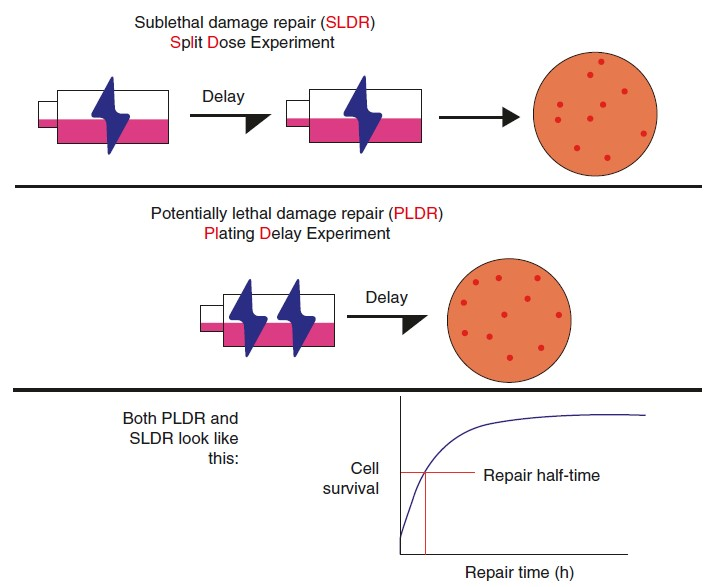
\includegraphics[width=0.6\textwidth]{Imagens/reparoDanosPontenciais.jpg}
		}%
		\caption{Quando a taxa de dose é inferior a 1 Gy por minuto, isso tem um efeito significativo na curva de sobrevivência das células mamíferas. Esse efeito é caracterizado pela presença de uma região inicial suave na curva, que indica resistência à radiação. Especificamente em taxas de dose abaixo de 1 Gy/min, ocorre uma significativa redução da morte celular induzida pela radiação de Baixa Transferência Linear de Energia (LET), resultando em maiores taxas de sobrevivência celular. Além disso, a inclinação da curva de sobrevivência se torna mais suave devido à ocorrência de reparo do DNA durante o período de irradiação. Esse processo de reparo permite a administração de várias doses físicas em Gy, mantendo uma maior sobrevivência celular.}
		\label{fig:reparoDanosPontenciais}
	\end{figure}

	O \textcolor{MediumOrchid}{\textbf{\textit{Reparo de Dano Subletal}}} refere-se aos \textcolor{MediumOrchid}{\textbf{\textit{danos que podem ser reparados pelas células}}} após a exposição à radiação. Nesse caso, as células têm a capacidade de corrigir ou recuperar os danos causados ao DNA e outras estruturas celulares. O SLDR ocorre quando as células ativam mecanismos de reparo para restaurar as lesões causadas pela radiação. Esse reparo pode ocorrer ao longo de um \textcolor{MediumOrchid}{\textbf{\textit{período de tempo}}} e é essencial para a sobrevivência e a recuperação das células irradiadas. Os testes que avaliam o SLDR são projetados para detectar a \textcolor{MediumOrchid}{\textbf{\textit{capacidade das células de se recuperarem}}} dos danos causados pela radiação.

	Por outro lado, o \textcolor{MediumOrchid}{\textbf{\textit{Reparo de Dano Potencialmente Letal}}} refere-se aos \textcolor{MediumOrchid}{\textbf{\textit{danos que não podem ser reparados pelas células}}} e podem levar à morte celular. Nesse caso, as lesões causadas pela radiação são tão graves que \textcolor{MediumOrchid}{\textbf{\textit{as células não conseguem recuperar sua função normal}}} e acabam morrendo. O PLDR é um tipo de dano mais grave e irreparável. Os testes que avaliam o PLDR são projetados para medir a \textcolor{MediumOrchid}{\textbf{\textit{capacidade das células de sobreviverem à radiação em longo prazo}}}, uma vez que o PLDR tem um impacto mais significativo na sobrevivência celular a longo prazo.

	Na prática da radioterapia, o intervalo de tempo entre as frações de tratamento é um aspecto importante a ser considerado. Geralmente, é necessário permitir um período de descanso entre as sessões para que o organismo se recupere dos efeitos da radiação e repare possíveis danos causados aos tecidos saudáveis circundantes.

	Na maioria dos \textcolor{MediumOrchid}{\textbf{\textit{regimes de radioterapia realizados duas vezes ao dia}}}, um intervalo mínimo de \textcolor{MediumOrchid}{\textbf{\textit{6 horas}}} é estabelecido entre as frações. Esse intervalo permite que o organismo tenha tempo suficiente para reparar danos celulares e minimizar os efeitos colaterais decorrentes da radiação. Manter um intervalo adequado também ajuda a preservar a saúde dos tecidos normais e reduzir a toxicidade associada ao tratamento.

	Para regimes de radioterapia realizados três vezes ao dia, um intervalo mínimo de 4 horas pode ser permitido. No entanto, é importante ressaltar que essa prática pode estar mais relacionada a considerações de agendamento do que a necessidades biológicas específicas. Embora um intervalo mais curto entre as frações possa ser viável em termos de agenda de tratamento, é fundamental garantir que seja suficiente para permitir uma recuperação adequada entre as sessões e evitar complicações desnecessárias.

	É importante destacar que esses intervalos mínimos são apenas diretrizes gerais e podem variar dependendo do tipo de câncer, da resposta individual do paciente à radiação e das características específicas do regime de tratamento prescrito. O planejamento e a programação das sessões de radioterapia levam em consideração diversos fatores, como o tipo e estágio do câncer, a tolerância dos tecidos saudáveis circundantes e a resposta do paciente ao tratamento.

	Em suma, estabelecer um intervalo adequado entre as frações de tratamento é fundamental para permitir a recuperação dos tecidos normais e otimizar os resultados terapêuticos. A determinação do intervalo de tempo entre as sessões é baseada em considerações clínicas, biológicas e logísticas, com o objetivo de alcançar um equilíbrio entre a eficácia do tratamento e a qualidade de vida do paciente.

\section{Efeito do Oxigênio}

	A \textcolor{MediumOrchid}{\textbf{\textit{Hipótese da Fixação do Oxigênio}}} é uma teoria que descreve os efeitos da radiação ionizante na presença de oxigênio. A radiação gera pares de íons na água, o que é um exemplo de ação indireta da radiação. Esses pares de íons reagem com moléculas, formando radicais livres dentro de nanossegundos após a ionização. Os antioxidantes, como o glutationa (GSH), são capazes de eliminar esses radicais livres em microssegundos. No entanto, quando o \textcolor{MediumOrchid}{\textbf{\textit{oxigênio está presente}}}, a hipótese afirma que ocorre uma \textcolor{MediumOrchid}{\textbf{\textit{reação adicional}}}: Os radicais livres gerados pela radiação reagem com o oxigênio, formando \textcolor{MediumOrchid}{\textbf{\textit{peróxidos}}} no DNA. Esses peróxidos são conhecidos como \textcolor{MediumOrchid}{\textbf{\textit{espécies reativas de oxigênio}}} (EROs) e são \textcolor{MediumOrchid}{\textbf{\textit{mais difíceis de serem reparados}}} pelas células em comparação aos danos causados diretamente pela radiação no DNA. A formação de peróxidos no DNA é chamada de \textcolor{MediumOrchid}{\textbf{\textit{"fixação do oxigênio"}}} e é um fenômeno que amplifica os efeitos indiretos da radiação ionizante (\ref{fig:hipoteseFixacaoOxigenio}).

	\begin{figure}[h]
		\centering
		\fcolorbox{DarkTurquoise}{white}{%
			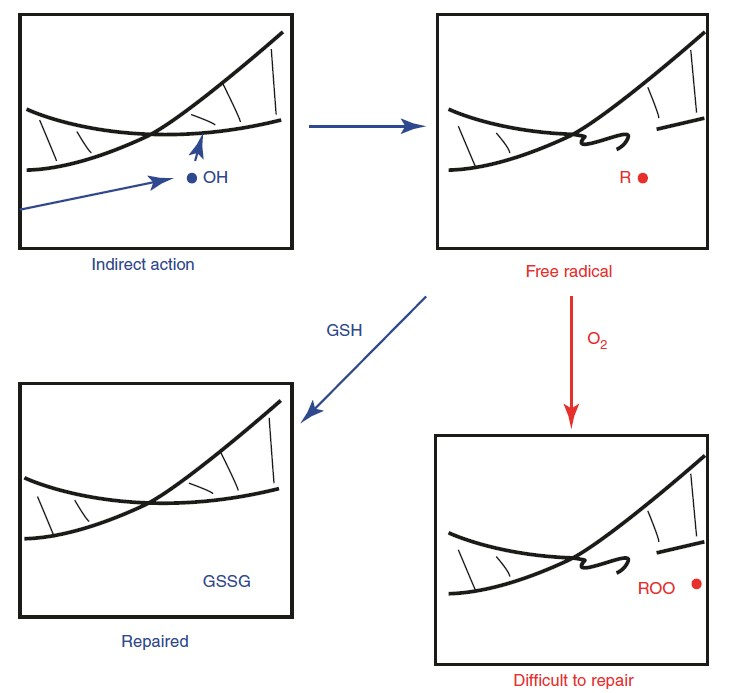
\includegraphics[width=0.5\textwidth]{Imagens/hipoteseFixacaoOxigenio.jpg}
		}%
		\caption{A hipótese da fixação de oxigênio. Os radicais livres são facilmente reparados por antioxidantes, mas o oxigênio molecular pode convertê-los em peróxidos que são mais difíceis de serem reparados.}
		\label{fig:hipoteseFixacaoOxigenio}
	\end{figure}

	É importante destacar que a \textcolor{MediumOrchid}{\textbf{\textit{concentração de oxigênio}}}, seja alta ou baixa, \textcolor{MediumOrchid}{\textbf{\textit{segundos antes ou depois da irradiação, não tem um impacto significativo no processo de fixação do oxigênio}}}. O que é crucial é a \textcolor{MediumOrchid}{\textbf{\textit{presença de oxigênio durante ou logo após a irradiação}}}. Além disso, a \textcolor{MediumOrchid}{\textbf{\textit{hipóxia transitória}}}, que se refere à privação temporária de oxigênio, desempenha um papel vital na radiobiologia. A \textcolor{MediumOrchid}{\textbf{\textit{ausência de oxigênio}}} durante a irradiação pode levar a uma menor formação de peróxidos no DNA, \textcolor{MediumOrchid}{\textbf{\textit{reduzindo assim os efeitos indiretos da radiação}}}.

\subsection*{Quantidade de Oxigênio Para Causar o Efeito do Oxigênio}

	O efeito do oxigênio pode ser observado mesmo em \textcolor{MediumOrchid}{\textbf{\textit{concentrações muito baixas}}}. A \textcolor{MediumOrchid}{\textbf{\textit{extensão}}} desse efeito depende da concentração de oxigênio presente no ambiente. Os exemplos abaixo sobre os níveis de oxigênio e seus efeitos correspondentes fornecem uma compreensão dos diferentes impactos do oxigênio em diferentes concentrações:

	\begin{exemplo}
		\begin{itemize}[label=\textcolor{CarnationPink}{$\blacktriangleright$}]
			\item Em \textcolor{DarkTurquoise}{\textbf{\textit{concentrações muito baixas de oxigênio}}}, como \SI{0.001}{\percent} (\SI{0.008}{\mmHg}), que representa uma condição completamente anóxica, não há um efeito significativo do oxigênio. Isso ocorre porque a quantidade de oxigênio presente é insuficiente para gerar reações com os radicais livres formados pela radiação ionizante.

			\item  Quando a \textcolor{DarkTurquoise}{\textbf{\textit{concentração de oxigênio aumenta para \SI{0.5}{\percent} (\SI{4}{\mmHg})}}}, ocorre um efeito do oxigênio, que é aproximadamente a metade do seu efeito máximo. 
			
			\item À medida que a \textcolor{DarkTurquoise}{\textbf{\textit{concentração de oxigênio aumenta para \SI{2}{\percent} (\SI{16}{\mmHg}), o efeito completo do oxigênio é observado}}}, e não há diferença significativa com aumentos adicionais na concentração de oxigênio. Nesse ponto, o oxigênio presente é suficiente para reagir com os radicais livres gerados pela radiação ionizante, resultando na formação de peróxidos no DNA.
		\end{itemize}
	\end{exemplo}
	
	É importante mencionar que esses níveis de oxigênio fornecidos como referência são para fornecer uma compreensão das concentrações de oxigênio em diferentes contextos fisiológicos e ambientais. 
	
	Tecidos completamente \textcolor{MediumOrchid}{\textbf{\textit{hipóxicos}}}, que têm um nível de oxigênio de \SI{0.13}{\percent} (\SI{1}{\mmHg}), normalmente são encontrados em situações patológicas ou em áreas de tumores com \textcolor{MediumOrchid}{\textbf{\textit{deficiência no suprimento sanguíneo}}}. O sangue venoso normalmente contém níveis de oxigênio entre \SIrange{2}{5}{\percent} (\SIrange{20}{40}{\mmHg}), enquanto o sangue arterial tem níveis de oxigênio entre \SIrange{8}{13}{\percent} (\SIrange{60}{100}{\mmHg}). O ar ambiente possui uma concentração de oxigênio de \SI{20}{\percent} (\SI{150}{\mmHg}), enquanto o oxigênio puro tem uma concentração de \SI{100}{\percent} (\SI{760}{\mmHg}).

	A \textcolor{MediumOrchid}{\textbf{\textit{hipóxia}}}, que se refere a \textcolor{MediumOrchid}{\textbf{\textit{níveis reduzidos de oxigênio}}} nos tecidos, confere um \textcolor{MediumOrchid}{\textbf{\textit{efeito protetor}}} aos tumores em relação aos danos induzidos pela radiação. Isso ocorre porque os tumores frequentemente apresentam um microambiente hipóxico, o que \textcolor{MediumOrchid}{\textbf{\textit{reduz sua sensibilidade ao oxigênio}}}. No entanto, é importante destacar que os tecidos normais não requerem condições hipóxicas para seu funcionamento ideal. Portanto, \textcolor{MediumOrchid}{\textbf{\textit{a hipóxia não oferece a mesma proteção aos tecidos normais}}} em relação aos efeitos da radiação, uma vez que sua função adequada depende de níveis de oxigênio adequados em condições fisiológicas normais.

\section{Oxygen Enhancement Ratio (OER)}

	A \textcolor{DarkTurquoise}{\textbf{\textit{Razão de Aprimoramento pelo Oxigênio}}} (OER, na sigla em inglês) é uma medida que descreve a \textcolor{MediumOrchid}{\textbf{\textit{sensibilidade relativa das células aos efeitos da radiação em diferentes níveis de oxigênio}}}. Ela é definida como a \textcolor{MediumOrchid}{\textbf{\textit{razão entre as doses necessárias para produzir o mesmo efeito biológico em condições hipóxicas e normóxicas}}}. A OER é uma ferramenta importante na radioterapia, pois nos ajuda a compreender a influência do oxigênio na resposta das células tumorais à radiação.

	\begin{equation}
		OER = \frac{\text{Dose (Hipóxia) para causar um efeito}}{\text{Dose (Normoxia) para causar o mesmo efeito}}
	\end{equation}

	\

	No caso dos \textcolor{MediumOrchid}{\textbf{\textit{fótons}}} de entorno de \SI{1}{\mega\electronvolt} (\SI{1}{\mega\volt}) -- \ce{^{60}Co} --, que são utilizados em radioterapia, um valor típico de OER é em torno de \textcolor{MediumOrchid}{\textbf{\textit{3.0}}}, variando de 2.5 a 3.5. Isso significa que, em condições completamente hipóxicas, seria necessário aplicar uma dose de \SI{6}{\gray} de radiação de \ce{^{60}Co} para alcançar o mesmo efeito biológico de uma dose de \SI{2}{\gray} de radiação de \ce{^{60}Co} em condições normóxicas. Essa diferença destaca o impacto significativo que a hipóxia pode ter na resposta dos tumores à radioterapia.

	Além disso, \textcolor{MediumOrchid}{\textbf{\textit{o valor do OER também pode ser influenciado pela fração de tratamento}}}, ou seja, o número de frações de radioterapia administradas. Em geral, alto tamanho de fração (hipofracionamento, onde uma dose mais alta de radiação é administrada em uma única fração) apresentam um OER ligeiramente maior ($\sim 3.5$) em comparação com pequenos tamanhos de fração(hiperfracionamento, onde a mesma dose total é entregue em múltiplas frações menores ) ($\sim 2.5$). Isso ocorre porque no \textcolor{MediumOrchid}{\textbf{\textit{hiperfracionamento}}}, \textcolor{MediumOrchid}{\textbf{\textit{a curva de sobrevida celular é dominada pelas células mais sensíveis na fase G2/M}}} do ciclo celular, que apresentam um \textcolor{MediumOrchid}{\textbf{\textit{OER mais baixo}}}. Em contraste, no \textcolor{MediumOrchid}{\textbf{\textit{hipofracionamento}}}, a curva de sobrevivência é dominada pelas \textcolor{MediumOrchid}{\textbf{\textit{células mais resistentes na fase S}}}, que têm um \textcolor{MediumOrchid}{\textbf{\textit{OER mais alto}}}. Essa relação entre o OER e a fração de tratamento é inversa à observada na Efetividade Biológica Relativa (RBE).

	Vale ressaltar que o valor do OER pode variar dependendo do \textcolor{MediumOrchid}{\textbf{\textit{tipo de radiação}}} utilizada. A radiação de Baixa Transferência Linear de Energia \textcolor{MediumOrchid}{\textbf{\textit{(baixa LET)}}}, que causa principalmente danos por ação indireta, apresenta um \textcolor{MediumOrchid}{\textbf{\textit{OER mais alto}}}, em torno de 3. Isso ocorre devido à \textcolor{MediumOrchid}{\textbf{\textit{dependência da radiação de baixa LET em relação ao oxigênio}}}. Em contraste, a radiação de \textcolor{MediumOrchid}{\textbf{\textit{Alta LET}}}, que causa mais danos por ação direta, tem um \textcolor{MediumOrchid}{\textbf{\textit{OER mais baixo}}}, em torno de 1, pois é menos dependente do oxigênio para produzir efeitos biológicos (\ref{fig:OER}). 

	\begin{figure}[h]
		\centering
		\fcolorbox{DarkTurquoise}{white}{%
			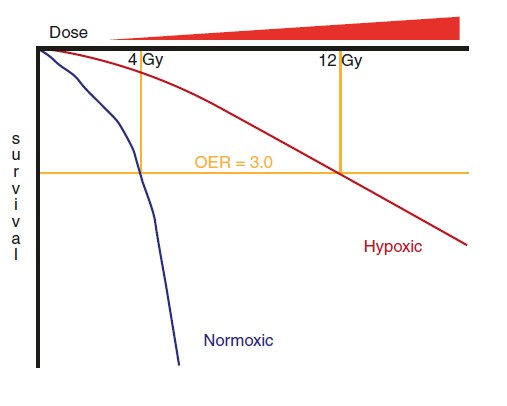
\includegraphics[width=0.6\textwidth]{Imagens/OER.jpg}
		}%
		\caption{A Razão de Aprimoramento pelo Oxigênio (OER) é definida como a razão entre as doses necessárias para alcançar o mesmo efeito, conforme indicado pela linha horizontal laranja no gráfico. Ela representa a diferença na resposta à radiação entre as condições normóxicas (com oxigênio) e hipóxicas (sem oxigênio). O OER quantifica o impacto do oxigênio na efetividade biológica da radiação.}
		\label{fig:OER}
	\end{figure}

	Em resumo, a Razão de Aprimoramento pelo Oxigênio (OER) é uma medida que descreve a sensibilidade das células à radiação em diferentes níveis de oxigênio. A hipóxia, ou falta de oxigênio, aumenta o valor do OER, tornando as células tumorais menos sensíveis à radioterapia.

\section{Efetividade Biológica Relativa}

	Nem todos os tipos de radiação têm a mesma Efetividade Biológica Relativa (RBE). O RBE é uma medida que \textcolor{MediumOrchid}{\textbf{\textit{compara a efetividade de uma radiação de teste em relação a uma radiação padrão na produção de um determinado efeito biológico}}}. Ele é definido como a \textcolor{MediumOrchid}{\textbf{\textit{razão entre as doses necessárias para alcançar o mesmo resultado biológico}}} com a radiação de teste em comparação com a radiação padrão.

	O RBE é geralmente medido com base em \textcolor{MediumOrchid}{\textbf{\textit{efeitos agudos}}}, como a eliminação de células. Ele compara a resposta das células irradiadas com a radiação de teste em relação à radiação padrão, que é comumente definida como \textcolor{MediumOrchid}{\textbf{\textit{raios-X de \SI{250}{\kilo\volt}}}} ou \textcolor{MediumOrchid}{\textbf{\textit{raios gama de \ce{^{60}Co}}}}. Por exemplo, se um determinado tipo de radiação tem um RBE de 3, isso significa que você precisaria aplicar \SI{3}{\gray} dessa radiação para obter o mesmo efeito de eliminação celular que \SI{1}{\gray} da radiação padrão (\ref{fig:rbe}).

	\begin{figure}[h]
		\centering
		\fcolorbox{DarkTurquoise}{white}{%
			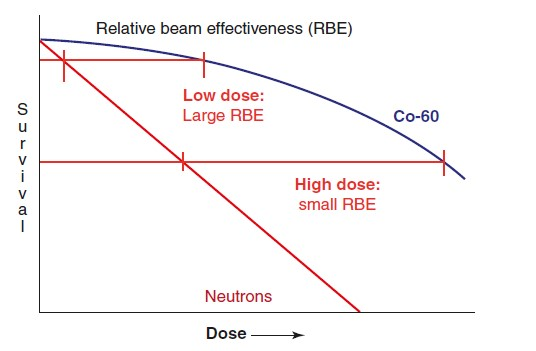
\includegraphics[width=0.5\textwidth]{Imagens/rbe.jpg}
		}%
		\caption{RBE e Dose: RBE é definido como a razão das doses que alcançam o mesmo efeito, conforme mostrado pela linha horizontal. RBE é maior em tamanhos de fração menores do que em tamanhos de fração maiores.}
		\label{fig:rbe}
	\end{figure}

	O valor do RBE pode \textcolor{MediumOrchid}{\textbf{\textit{variar}}} dependendo do \textcolor{MediumOrchid}{\textbf{\textit{tipo de célula}}} irradiada. Células \textcolor{MediumOrchid}{\textbf{\textit{radiorresistentes}}}, que já são naturalmente resistentes à radiação, podem apresentar \textcolor{MediumOrchid}{\textbf{\textit{valores de RBE mais altos para radiações de alta LET}}}. Isso ocorre porque a radiação de alta LET, como os feixes de partículas pesadas, como prótons ou íons de carbono, causa danos mais complexos no DNA, que são mais difíceis de reparar, mesmo em células radiorresistentes.

	Por outro lado, \textcolor{MediumOrchid}{\textbf{\textit{células muito sensíveis à radiação}}}, incluindo aquelas com mutações nas vias de reparo de quebras de dupla fita do DNA, podem ser mais sensíveis à radiação padrão, como raios-X ou gama de baixa LET, resultando em \textcolor{MediumOrchid}{\textbf{\textit{valores de RBE mais baixos para radiação de alta LET}}}. Isso ocorre porque essas células já têm dificuldade em reparar danos no DNA causados pela radiação padrão, e a radiação de alta LET não fornece benefícios adicionais na indução de danos.

	O RBE também pode ser influenciado pela \textcolor{MediumOrchid}{\textbf{\textit{taxa de dose}}} e pela \textcolor{MediumOrchid}{\textbf{\textit{fração do tratamento}}}. Em geral, o RBE tende a ser \textcolor{MediumOrchid}{\textbf{\textit{maior}}} em \textcolor{MediumOrchid}{\textbf{\textit{hiperfracionamento}}}, onde os mecanismos de reparo das células são mais eficazes para a radiação padrão de \textcolor{MediumOrchid}{\textbf{\textit{baixa LET}}}. Porém, para radiação de \textcolor{MediumOrchid}{\textbf{\textit{alta LET}}}, esses mecanismos de reparo são menos eficazes, resultando em um \textcolor{MediumOrchid}{\textbf{\textit{RBE mais baixo}}}. Em \textcolor{MediumOrchid}{\textbf{\textit{hipofracionamento}}}, o RBE tende a ser \textcolor{MediumOrchid}{\textbf{\textit{menor}}}, uma vez que as células têm \textcolor{MediumOrchid}{\textbf{\textit{menos tempo para reparar os danos}}} causados pela radiação padrão de \textcolor{MediumOrchid}{\textbf{\textit{baixa LET}}}.

	É importante diferenciar o RBE do \textcolor{MediumOrchid}{\textbf{\textit{Fator de Qualidade}}} (QF), também conhecido como Fator de Ponderação (WR), que é usado para fins de proteção radiológica. O QF é um \textcolor{MediumOrchid}{\textbf{\textit{valor atribuído a diferentes tipos de radiação com base em suas características físicas, biológicas e potencial de dano}}}. Ele é usado para calcular a \textcolor{MediumOrchid}{\textbf{\textit{dose equivalente}}} em termos de risco para tecidos normais e efeitos tardios, como carcinogênese e riscos hereditários. O QF é uma \textcolor{MediumOrchid}{\textbf{\textit{estimativa conservadora}}} que \textcolor{MediumOrchid}{\textbf{\textit{superestima}}} o efeito da radiação de partículas em comparação com a radiação de baixa LET, para garantir uma margem de segurança na proteção radiológica.

\section{LET}

	Na radiobiologia e proteção radiológica, a transferência linear de energia (LET) é uma quantidade física crucial usada para caracterizar a qualidade de um feixe de radiação ionizante. Ao contrário do poder de freamento, que se concentra na perda de energia de uma partícula carregada energeticamente à medida que se move através de um meio, a \textcolor{MediumOrchid}{\textbf{\textit{LET}}} enfatiza a \textcolor{MediumOrchid}{\textbf{\textit{taxa linear de absorção de energia pelo meio}}} à medida que a partícula carregada o atravessa.

	A Comissão Internacional de Unidades e Medidas de Radiação (ICRU) define o LET da seguinte forma: \textit{"O LET de partículas carregadas em um meio é o quociente $dE/dl$, onde $dE$ é a energia média localmente transmitida ao meio por uma partícula carregada de energia especificada ao percorrer uma distância $dl$."}

	Enquanto o poder de freamento é geralmente expresso em unidades de MeV/cm, a unidade padrão usada para o LET é keV/$\mu$m. A energia média é determinada dividindo-se a trajetória da partícula em incrementos de energia iguais e calculando o comprimento médio da trajetória em que esses incrementos de energia são depositados.

	\

	\begin{tcolorbox}[width=\textwidth, colback={white}, colbacktitle={DarkTurquoise!50!white}, title={$\bigstar$ \LobsterTwo{Valores Típicos da LET} $\bigstar$}, coltitle={CarnationPink}, colframe={DarkTurquoise}, fonttitle=\rmfamily\bfseries\Large, breakable]\label{exp:let}
	\textcolor{MediumOrchid}{\LobsterTwo\large\textbf{Baixa LET:}}
	\begin{itemize}
		\item \textcolor{DarkTurquoise}{\textbf{\textit{Prótons de 10 MeV}}}: 5 keV/$\mu$m
		\item \textcolor{DarkTurquoise}{\textbf{\textit{Raios X de 250 kVp}}}: 2 keV/$\mu$m		
		\item \textcolor{DarkTurquoise}{\textbf{\textit{Prótons de 150 MeV}}}: 0.5 keV/$\mu$m
		\item \textcolor{DarkTurquoise}{\textbf{\textit{Raios $\gamma$ de Cobalto-60}}}: 0.3 keV/$\mu$m
		\item \textcolor{DarkTurquoise}{\textbf{\textit{Raios X de 3 MeV}}}: 0.3 keV/$\mu$m
		\item \textcolor{DarkTurquoise}{\textbf{\textit{Elétrons de 10 keV}}}: 2.3 keV/$\mu$m
		\item \textcolor{DarkTurquoise}{\textbf{\textit{Elétrons de 1 MeV}}}: 0.25 keV/$\mu$m
	\end{itemize}

	\textcolor{MediumOrchid}{\LobsterTwo\large\textbf{Alta LET:}}
	\begin{itemize}
		\item \textcolor{DarkTurquoise}{\textbf{\textit{Nêutrons de 14 MeV}}}: 12 keV/$\mu$m
		\item \textcolor{DarkTurquoise}{\textbf{\textit{Elétrons de 1 keV}}}: 12.3 keV/$\mu$m
		\item \textcolor{DarkTurquoise}{\textbf{\textit{Prótons de 2 MeV}}}: 17 keV/$\mu$m
		\item \textcolor{DarkTurquoise}{\textbf{\textit{Íons de Carbono com 100 MeV}}}: 160 keV/$\mu$m
		\item \textcolor{DarkTurquoise}{\textbf{\textit{Partículas carregadas pesadas}}}: 100-2000 keV/$\mu$m
	\end{itemize}

	\end{tcolorbox}

	\
	
	Raios X e raios $\gamma$ são considerados radiações de baixo LET (esparsadamente ionizantes), enquanto nêutrons energéticos, prótons e partículas carregadas pesadas são radiações de alto LET (densamente ionizantes). \textcolor{MediumOrchid}{\textbf{\textit{O valor de demarcação entre LET baixo e alto é aproximadamente 10 keV/$\mu$m}}}.

\section{Relação entre Transferência Linear de Energia (LET), RBE e OER}

	LET, ou Transferência Linear de Energia, é uma medida importante na caracterização de feixes de radiação, pois está relacionada à capacidade da radiação de depositar energia em um meio através de ionizações (\ref{fig:efeitoLetAltaEBaixe}). a LET é definido como a energia média depositada por unidade de comprimento ao longo da trajetória da radiação. Valores mais altos de LET indicam que a radiação possui uma maior densidade de ionizações ao longo de sua trajetória.

	\begin{figure}[!h]
		\centering
		\fcolorbox{DarkTurquoise}{white}{%
			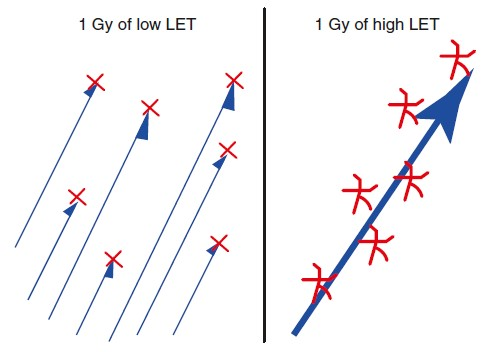
\includegraphics[width=0.6\textwidth]{Imagens/efeitoLetAltaEBaixe.jpg}
		}%
		\caption{O diagrama ilustra a diferença entre radiação de Baixa Transferência Linear de Energia (LET) e radiação de Alta Transferência Linear de Energia. Ambos os tipos de radiação depositam a mesma quantidade de dose de radiação, representada pelas estrelas vermelhas indicando ionizações. No entanto, há uma diferença distinta na distribuição dos eventos de ionização. No caso da radiação de baixa LET, os eventos de ionização estão amplamente dispersos por toda a área-alvo. As partículas ionizantes ou fótons atravessam o meio com menor interação, resultando em um padrão mais difuso de ionizações. Por outro lado, a radiação de alta LET apresenta uma trilha densa de eventos de ionização. As partículas ionizantes ou fótons depositam sua energia de forma concentrada ao longo de uma trilha estreita no meio. Essa trilha densa de ionizações é característica da radiação de alta LET. Os padrões contrastantes de ionizações entre radiação de baixo e alta LET refletem suas diferentes interações físicas com o meio. A radiação de baixa LET interage menos frequentemente com o meio, resultando em eventos de ionização dispersos e menos densamente concentrados. Em contraste, a radiação de alta LET passa por interações mais frequentes e em curta distância, resultando em uma trilha densa de eventos de ionização espaçados de perto. É importante observar que a distinção entre radiação de baixo e alta LET tem implicações para seus efeitos biológicos e efetividade relativa na eliminação de células. A radiação de alta LET, com seus eventos de ionização concentrados, pode causar danos mais significativos em estruturas biológicas, incluindo o DNA, em comparação com a radiação de baixa LET..}
		\label{fig:efeitoLetAltaEBaixe}
	\end{figure}

	a LET desempenha um papel importante na radiobiologia, uma vez que afeta a interação da radiação com a matéria e os tecidos biológicos. À medida que a \textcolor{MediumOrchid}{\textbf{\textit{LET aumenta}}}, a \textcolor{MediumOrchid}{\textbf{\textit{Efetividade Biológica Relativa (RBE) da radiação também tende a aumentar}}} até atingir um pico em torno de \textcolor{MediumOrchid}{\textbf{\textit{100 keV/\mu m}}}.

	O \textcolor{MediumOrchid}{\textbf{\textit{``overkill effect''}}} é um fenômeno observado quando a \textcolor{MediumOrchid}{\textbf{\textit{densidade de ionizações causada por radiação de alta LET excede a quantidade necessária para causar a morte celular}}}. Nesse caso, a radiação se torna \textcolor{MediumOrchid}{\textbf{\textit{menos eficaz}}} na eliminação de células por dose absorvida. Isso ocorre porque, com uma alta densidade de ionizações, a radiação pode causar danos excessivos nas células, ultrapassando o limite necessário para a morte celular. Esse excesso de danos pode levar a uma menor eficácia na eliminação de células, uma vez que a capacidade de reparo das células é sobrecarregada. 

	Além disso, à medida que a \textcolor{MediumOrchid}{\textbf{\textit{LET aumenta}}}, a \textcolor{MediumOrchid}{\textbf{\textit{ação direta}}} da radiação, que envolve a interação direta das partículas com o DNA, torna-se mais \textcolor{MediumOrchid}{\textbf{\textit{dominante}}} em relação à ação indireta, que envolve a ionização de moléculas de água e a formação de radicais livres. A \textcolor{MediumOrchid}{\textbf{\textit{ação direta}}} é \textcolor{MediumOrchid}{\textbf{\textit{menos dependente}}} da presença de \textcolor{MediumOrchid}{\textbf{\textit{oxigênio}}}, o que significa que a \textcolor{MediumOrchid}{\textbf{\textit{radiação de alta LET pode ser mais eficaz na eliminação de células mesmo em condições hipóxicas}}}.

	No entanto, além de \textcolor{MediumOrchid}{\textbf{\textit{100 keV/\mu m}}}, o \textcolor{MediumOrchid}{\textbf{\textit{RBE começa a diminuir à medida que a LET continua aumentando}}}. Isso é conhecido como \textcolor{MediumOrchid}{\textbf{\textit{``efeito de superdosagem''}}}. Nesse ponto, a densidade de ionizações entregue pelas partículas se torna excessiva em relação ao que é necessário para induzir a morte celular, resultando em menos células mortas por unidade de dose absorvida. Portanto, o \textcolor{MediumOrchid}{\textbf{\textit{RBE atinge seu valor máximo em torno de 100 keV/\mu m, e depois diminui à medida que a LET aumenta}}} ainda mais.

	A \textcolor{MediumOrchid}{\textbf{\textit{razão de Aprimoramento pelo Oxigênio (OER)}}} apresenta uma \textcolor{MediumOrchid}{\textbf{\textit{relação inversa}}} com a \textcolor{MediumOrchid}{\textbf{\textit{LET}}}. O \textcolor{MediumOrchid}{\textbf{\textit{OER é maior em baixos valores de LET}}}, normalmente abaixo de \textcolor{MediumOrchid}{\textbf{\textit{1 keV/\mu m}}}, onde está na faixa de 2.5 a 3.5. Isso indica um aumento no efeito do oxigênio na sensibilidade da radiação. À medida que a \textcolor{MediumOrchid}{\textbf{\textit{LET aumenta}}}, o \textcolor{MediumOrchid}{\textbf{\textit{OER diminui e se aproxima de 1.0 para valores de LET acima de 100 keV/\mu m}}}. Isso significa que o oxigênio tem menos influência nos efeitos da radiação de alta LET. Essa diminuição no OER está relacionada à ação direta da radiação de alta LET, que é menos dependente do oxigênio para causar danos ao DNA. Portanto, à medida que a LET aumenta, a dependência do oxigênio nos efeitos da radiação diminui, levando a um OER mais baixo. A \ref{fig:OerERbe} apresenta a relação entre a LET, OER e RBE.

	\begin{figure}[h]
		\centering
		\fcolorbox{DarkTurquoise}{white}{%
			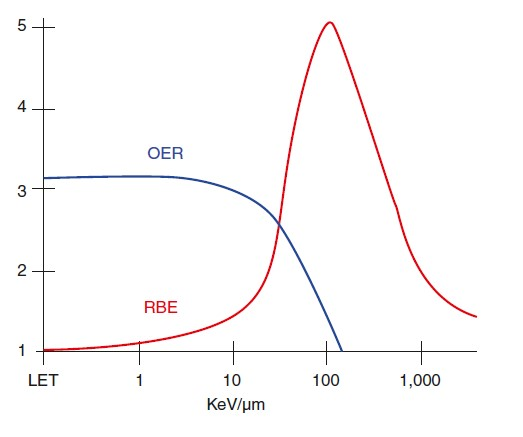
\includegraphics[width=0.6\textwidth]{Imagens/OerERbe.jpg}
		}%
		\caption{À medida que a Transferência Linear de Energia (LET) aumenta, tanto o Efeito de Aprimoramento pelo Oxigênio (OER - Oxygen Enhancement Ratio) quanto a Efetividade Biológica Relativa (RBE - Relative Biological Effectiveness) exibem relações distintas: O RBE geralmente aumenta com o aumento da LET até atingir um pico em torno de aproximadamente 100 keV/$\mu$m. Isso significa que a efetividade relativa da radiação em produzir efeitos biológicos aumenta com um LET mais alto até esse ponto. No entanto, para valores de LET acima desse pico, o RBE tende a diminuir com maiores aumentos na LET. Por outro lado, o OER tende a diminuir à medida que a LET aumenta, até atingir um valor próximo a 1 em torno de aproximadamente 100 keV/$\mu$m. O OER é uma medida do grau em que a presença de oxigênio afeta a resposta à radiação. Um OER mais baixo indica que a radiação é menos dependente da presença de oxigênio para produzir efeitos biológicos. Acima de 100 keV/$\mu$m, o OER permanece em torno de 1, indicando que a resposta à radiação não é mais influenciada significativamente pela presença de oxigênio..}
		\label{fig:OerERbe}
	\end{figure}

	Os \hyperref[exp:let]{valores de LET} podem variar dependendo do tipo de radiação. Para \textcolor{MediumOrchid}{\textbf{\textit{raios X}}}, \textcolor{MediumOrchid}{\textbf{\textit{raios gama}}} e \textcolor{MediumOrchid}{\textbf{\textit{elétrons}}} de megavoltagem, geralmente encontramos valores de LET entre \textcolor{MediumOrchid}{\textbf{\textit{0.2 e 0.5 keV/$\mu$m}}}. \textcolor{MediumOrchid}{\textbf{\textit{Prótons}}} rápidos com energia de \textcolor{MediumOrchid}{\textbf{\textit{150 MeV}}} têm um LET de \textcolor{MediumOrchid}{\textbf{\textit{0.5 keV/$\mu$m}}}. Já os \textcolor{MediumOrchid}{\textbf{\textit{raios X e raios gama}}} de kilovoltagem têm valores de LET entre \textcolor{MediumOrchid}{\textbf{\textit{2 e 4 keV/$\mu$m}}}. \textcolor{MediumOrchid}{\textbf{\textit{Prótons}}} lentos com energia de 10 MeV apresentam um LET de aproximadamente \textcolor{MediumOrchid}{\textbf{\textit{5 keV/$\mu$m}}}.

	Para partículas de maior massa, como nêutrons rápidos e partículas alfa, os valores de LET são mais elevados, em torno de 100 keV/$\mu$m. Íons pesados, como carbono, argônio, oxigênio e ferro, têm valores ainda mais altos de LET, variando de 100 a 1000 keV/$\mu$m.

	No caso dos \textcolor{MediumOrchid}{\textbf{\textit{íons de carbono}}} utilizados em terapia, a \textcolor{MediumOrchid}{\textbf{\textit{LET pode variar ao longo do pico de Bragg estendido (SOBP)}}}, que é a região de deposição de energia ao longo da trajetória do feixe. Os valores de LET aumentam de aproximadamente \textcolor{MediumOrchid}{\textbf{\textit{20 keV/$\mu$m}}} na \textcolor{MediumOrchid}{\textbf{\textit{borda proximal}}} do SOBP para cerca de \textcolor{MediumOrchid}{\textbf{\textit{100 keV/$\mu$m}}} na borda distal.

	Em resumo, a LET é uma medida da capacidade da radiação de depositar energia em um meio. À medida que a LET aumenta, a efetividade biológica da radiação também tende a aumentar até atingir um pico em torno de 100 keV/\mu m. No entanto, além desse ponto, o RBE começa a diminuir devido ao efeito de superdosagem. Os valores de LET variam dependendo do tipo de radiação, e para a terapia com íons de carbono, a LET pode variar ao longo do Spread-Out Bragg Peak.

\section{Microambiente Tumoral}

\subsection*{Vasculatura Tumoral}

	A vasculatura tumoral desempenha um papel crucial no crescimento e na progressão dos tumores. Para \textcolor{MediumOrchid}{\textbf{\textit{sobreviver}}} e se \textcolor{MediumOrchid}{\textbf{\textit{expandi}}}r, os tumores precisam de um \textcolor{MediumOrchid}{\textbf{\textit{suprimento sanguíneo}}} que forneça \textcolor{MediumOrchid}{\textbf{\textit{oxigênio}}} e nutrientes. A \textcolor{DarkTurquoise}{\textbf{\textit{angiogênese}}}, processo de \textcolor{MediumOrchid}{\textbf{\textit{formação de novos vasos sanguíneos a partir dos vasos pré-existentes}}}, é fundamental para permitir que os tumores estabeleçam seu próprio suprimento vascular.

	Os tumores frequentemente crescem em \textcolor{MediumOrchid}{\textbf{\textit{padrões de aglomerados}}} ou cordões, com parte do tecido estromal normal ao seu redor, o que lhes proporciona a oportunidade de se \textcolor{MediumOrchid}{\textbf{\textit{conectar aos vasos sanguíneos}}} existentes. Além disso, os tumores podem \textcolor{MediumOrchid}{\textbf{\textit{secretar fatores de crescimento}}}, como o fator de crescimento endotelial vascular (VEGF), que estimulam a formação de novos vasos sanguíneos. O VEGF é um importante fator de crescimento angiogênico e tem sido alvo de medicamentos como o bevacizumabe (Avastin) e outras terapias antiangiogênicas.

	A \textcolor{MediumOrchid}{\textbf{\textit{vasculatura}}} dentro dos tumores apresenta \textcolor{MediumOrchid}{\textbf{\textit{características anormais}}}, como \textcolor{MediumOrchid}{\textbf{\textit{permeabilidade aumentada}}}, \textcolor{MediumOrchid}{\textbf{\textit{organização deficiente}}} e \textcolor{MediumOrchid}{\textbf{\textit{funcionalidade reduzida}}} em comparação com os vasos sanguíneos normais. Essa rede vascular aberrante pode contribuir para a \textcolor{MediumOrchid}{\textbf{\textit{oxigenação inadequada do tumor}}} e para a entrega limitada de agentes terapêuticos às células tumorais. No entanto, a \textcolor{MediumOrchid}{\textbf{\textit{hipótese de normalização}}} sugere que a \textcolor{MediumOrchid}{\textbf{\textit{terapia antiangiogênica}}} pode ajudar a melhorar a \textcolor{MediumOrchid}{\textbf{\textit{perfusão do tumor}}}, eliminando os vasos sanguíneos anormais e promovendo a formação de vasos mais funcionais. Esse processo de normalização vascular pode melhorar a oxigenação e a entrega de medicamentos ao tumor, potencialmente aprimorando os resultados do tratamento.

	Em muitos tumores, existem \textcolor{MediumOrchid}{\textbf{\textit{regiões de necrose}}}, onde os \textcolor{MediumOrchid}{\textbf{\textit{níveis de oxigênio são extremamente baixos}}}, resultando na \textcolor{MediumOrchid}{\textbf{\textit{morte celular por falta de oxigênio (anóxia)}}}. A \textcolor{MediumOrchid}{\textbf{\textit{hipóxia}}}, caracterizada por baixos níveis de oxigênio, é conhecida por \textcolor{MediumOrchid}{\textbf{\textit{reduzir significativamente a eficácia da radiação de baixa transferência linear de energia (LET)}}}. As células tumorais hipóxicas são menos sensíveis aos danos causados pela radiação e podem ser mais resistentes ao tratamento. Estratégias estão sendo estudadas para superar a hipóxia, como técnicas de oxigenação ou terapias direcionadas à hipóxia, com o objetivo de melhorar os resultados da radioterapia.

\subsection*{A hipótese de Thomlinson-Gray}

	A \textcolor{DarkTurquoise}{\textbf{\textit{hipótese de Thomlinson-Gray}}}, proposta por Thomlinson e Gray em 1955, fornece informações  sobre os \textcolor{MediumOrchid}{\textbf{\textit{padrões de crescimento e oxigenação de tumores sólidos}}}, com foco especial em cânceres de pulmão em humanos. Essa hipótese foi formulada com base em observações e experimentos realizados por esses pesquisadores.

	De acordo com a hipótese de Thomlinson-Gray, tumores com diâmetro maior que aproximadamente 200 \mu m consistem em cordões tumorais cercados por estroma normal vascularizado. Dentro desses cordões tumorais, existe um núcleo necrótico. Foi observado que apenas os 100 \mu m mais externos do cordão tumoral contêm células viáveis, enquanto a porção interna é necrótica (\ref{fig:hipoteseThomlinsonGray}).

	\begin{figure}[h]
		\centering
		\fcolorbox{DarkTurquoise}{white}{%
			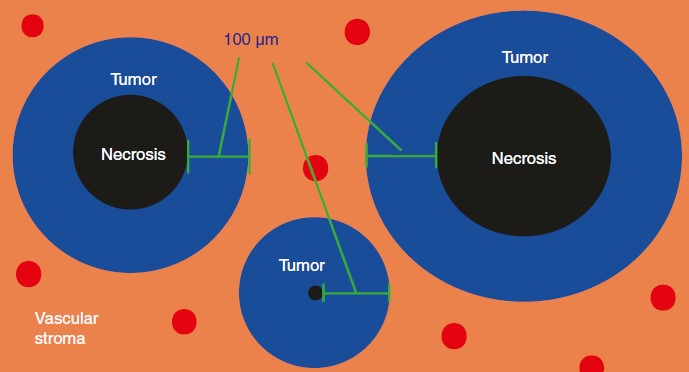
\includegraphics[width=0.5\textwidth]{Imagens/hipoteseThomlinsonGray.jpg}
		}%
		\caption{A hipótese de Thomlinson–Gray afirma que os tumores crescem em cordões ou aglomerados de células cercados por estroma normal. Independentemente do tamanho do cordão, apenas a camada mais externa, com aproximadamente 100 \mu m de espessura, contém células viáveis. Essa viabilidade limitada é atribuída à distância de difusão do oxigênio.}
		\label{fig:hipoteseThomlinsonGray}
	\end{figure}

	A hipótese propõe que a \textcolor{MediumOrchid}{\textbf{\textit{espessura do tecido tumoral viável seja limitada pela difusão de oxigênio}}}. O oxigênio é essencial para a sobrevivência e o funcionamento adequado das células. A \textcolor{MediumOrchid}{\textbf{\textit{distância de difusão do oxigênio}}} é estimada em cerca de \textcolor{MediumOrchid}{\textbf{\textit{70 \mu m}}}, além da qual a tensão de oxigênio diminui significativamente. Consequentemente, dentro da faixa de \textcolor{MediumOrchid}{\textbf{\textit{70 a 100 \mu m}}}, as células experimentam \textcolor{MediumOrchid}{\textbf{\textit{hipóxia crônica}}}, ou seja, são cronicamente privadas de um suprimento adequado de oxigênio. Além do limite de 100 \mu m, as células começam a morrer de \textcolor{MediumOrchid}{\textbf{\textit{anóxia}}}, que é a completa ausência de oxigênio. Isso leva à formação de um \textcolor{MediumOrchid}{\textbf{\textit{núcleo necrótico}}} dentro do tumor.

	Desde a proposta inicial da hipótese de Thomlinson-Gray, numerosos experimentos envolvendo a medição dos níveis de oxigênio dentro dos tumores têm fornecido suporte para sua validade. Esses estudos confirmaram a \textcolor{MediumOrchid}{\textbf{\textit{presença de regiões hipóxicas dentro dos tumores e o desenvolvimento de um núcleo necrótico além de uma determinada distância dos vasos sanguíneos}}}.

	Compreender a difusão limitada de oxigênio e a presença de regiões hipóxicas dentro dos tumores é crucial para o desenvolvimento de estratégias terapêuticas que possam superar os desafios relacionados à hipóxia no tratamento do câncer. Diversas abordagens estão sendo exploradas para melhorar a oxigenação das regiões tumorais hipóxicas e aumentar a eficácia da radioterapia e de outros tratamentos. Isso inclui o uso de técnicas de aumento de oxigênio, terapias direcionadas à hipóxia e tratamentos combinados, visando melhorar a oxigenação e potencializar a resposta do tumor ao tratamento.

\subsection*{Curvas mistas de Sobrevivência Normóxicas/Hipóxicas}

	Um \textcolor{MediumOrchid}{\textbf{\textit{tumor experimental}}} em um animal, semelhante a um tumor humano, é composto por \textcolor{MediumOrchid}{\textbf{\textit{células tumorais tanto normóxicas quanto hipóxicas}}}. Para avaliar as taxas de sobrevivência, o tumor é irradiado e as células são cultivadas, resultando em uma curva de sobrevivência apresentada na \ref{fig:medidaDiretaHipoxia}.

	\begin{figure}[h]
		\centering
		\fcolorbox{DarkTurquoise}{white}{%
			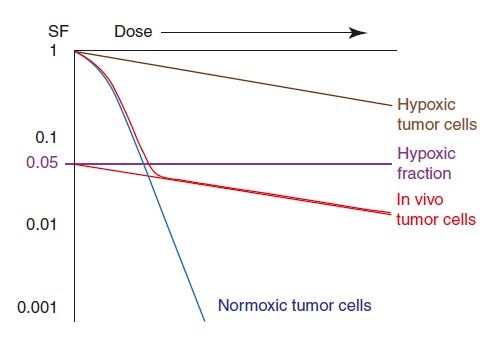
\includegraphics[width=0.5\textwidth]{Imagens/medidaDiretaHipoxia.jpg}
		}%
		\caption{Curva de sobrevivência in vivo: Tumores em um animal experimental foram irradiados e, posteriormente, as células foram cultivadas para determinar a sobrevivência celular (em vermelho). A curva de sobrevivência resultante pode ser conceituada como a combinação de duas curvas distintas: uma que representa a sobrevivência das células tumorais normóxicas (em azul) e outra que representa a sobrevivência das células tumorais hipóxicas (em marrom).}
		\label{fig:medidaDiretaHipoxia}
	\end{figure}

	O padrão ``bifásico'' observado na curva de sobrevivência do tumor, com duas regiões distintas, é uma característica comum encontrada em muitos tumores sólidos. Essas duas regiões correspondem às células normóxicas e hipóxicas presentes no tumor. \textcolor{MediumOrchid}{\textbf{\textit{Na região de baixa dose}}} \textcolor{MediumOrchid}{\textbf{\textit{o número de células normóxicas superam o número de células hipóxicas e, portanto, a curva de sobrevivência se assemelha mais a uma curva de sobrevivência normóxica.}}}. Isso ocorre porque as células normóxicas têm acesso a um suprimento adequado de oxigênio, que aumenta sua sensibilidade à radiação. Na região de \textcolor{MediumOrchid}{\textbf{\textit{altas doses}}}, as células normóxicas são totalmente eliminadas e as \textcolor{MediumOrchid}{\textbf{\textit{células hipóxicas}}}, que são menos sensíveis à radiação devido à falta de oxigênio, predominam fazendo com que a \textcolor{MediumOrchid}{\textbf{\textit{curva de sobrevivência se assemelhe mais a uma curva de sobrevivência hipóxica}}}.

	Ao extrapolar o segmento hipóxico da curva de sobrevivência para uma dose de radiação zero, é possível estimar a \textcolor{MediumOrchid}{\textbf{\textit{fração hipóxica}}}. A interseção da curva com o eixo Y, especificamente para o exemplo onde a fração de sobrevivência (SF) é igual a 0.05, indica que cerca de 5\% das células tumorais são hipóxicas. Esse valor é importante para compreender a contribuição relativa das células hipóxicas para a resistência do tumor à radiação.

	A Razão de Aprimoramento de Oxigênio \textcolor{MediumOrchid}{\textbf{\textit{(OER)}}} é um parâmetro que quantifica a sensibilidade relativa das células tumorais normóxicas e hipóxicas à radiação. O método de \textcolor{MediumOrchid}{\textbf{\textit{Powers-Tolmach}}} é comumente usado para esse calcular a OER comparando-se o \textcolor{MediumOrchid}{\textbf{\textit{$D_0$}}}, que é a dose necessária para reduzir a sobrevivência em 37\%, para as duas regiões da curva de sobrevivência, região de alta dose e de baixa dose. Por exemplo: com um \textcolor{MediumOrchid}{\textbf{\textit{$D_0$ de baixa dose de \SI{1.1}{\gray}}}} e um \textcolor{MediumOrchid}{\textbf{\textit{$D_0$ de alta dose de \SI{2.6}{\gray}}}}, o OER é determinado como \textcolor{MediumOrchid}{\textbf{\textit{$\text{OER} = 2.6/1.1 = 2.4$}}}. Isso significa que as células hipóxicas são cerca de 2.4 vezes mais resistentes à radiação em comparação com as células normóxicas.

\subsection*{Hipóxia Transitória e Crônica}

	A \textcolor{MediumOrchid}{\textbf{\textit{hipóxia transitória e crônica}}} são dois estados de privação de oxigênio que as células tumorais podem experimentar devido a \textcolor{MediumOrchid}{\textbf{\textit{distúrbios na vascularização do tumor}}}. Esses estados têm implicações significativas na resposta do tumor à radiação e no seu comportamento biológico.

	A \textcolor{DarkTurquoise}{\textbf{\textit{hipóxia transitória}}} ocorre quando os \textcolor{MediumOrchid}{\textbf{\textit{vasos sanguíneos}}} que fornecem oxigênio ao tumor são \textcolor{MediumOrchid}{\textbf{\textit{temporariamente bloqueados ou comprometidos}}}, levando a uma \textcolor{MediumOrchid}{\textbf{\textit{redução aguda do suprimento de oxigênio}}} para as células tumorais. Durante esse período, as células tumorais que estão localizadas nas proximidades dos vasos bloqueados enfrentam um ambiente hipóxico e exibem \textcolor{MediumOrchid}{\textbf{\textit{resistência à radiação}}}. A hipóxia transitória é uma \textcolor{MediumOrchid}{\textbf{\textit{resposta adaptativa}}} das células tumorais à falta de oxigênio, permitindo sua \textcolor{MediumOrchid}{\textbf{\textit{sobrevivência temporária}}} em condições adversas. No entanto, assim que o fluxo sanguíneo é restabelecido e o oxigênio é novamente fornecido às células, elas se tornam completamente oxigenadas e retomam sua atividade metabólica normal. O período de hipóxia transitória pode resultar em uma menor eficácia da radiação .

	Já a \textcolor{DarkTurquoise}{\textbf{\textit{hipóxia crônica}}} ocorre quando as \textcolor{MediumOrchid}{\textbf{\textit{células tumorais estão localizadas a uma distância considerável dos vasos sanguíneos funcionais}}}. Essas células experimentam uma \textcolor{MediumOrchid}{\textbf{\textit{privação prolongada de oxigênio}}}, resultando em hipóxia contínua. A hipóxia crônica é mais desafiadora, pois as células hipóxicas não têm acesso regular a um suprimento adequado de oxigênio. Essas células hipóxicas exibem \textcolor{MediumOrchid}{\textbf{\textit{resistência à radiação}}} devido à falta de oxigênio, o que dificulta sua resposta ao tratamento radioterápico. Além disso, a \textcolor{MediumOrchid}{\textbf{\textit{exposição prolongada à hipóxia crônica}}} pode levar à \textcolor{MediumOrchid}{\textbf{\textit{morte celular}}} ou à \textcolor{MediumOrchid}{\textbf{\textit{deterioração da viabilidade}}} das células tumorais. Por outro lado, a hipóxia crônica também pode desencadear \textcolor{MediumOrchid}{\textbf{\textit{adaptações genéticas}}} nas células tumorais e promover a \textcolor{MediumOrchid}{\textbf{\textit{seleção de subpopulações de células mais agressivas}}}, aumentando a probabilidade de metástase.

	As células tumorais têm \textcolor{MediumOrchid}{\textbf{\textit{mecanismos}}} para superar a hipóxia crônica. Um desses mecanismos é a \textcolor{MediumOrchid}{\textbf{\textit{angiogênese}}}, que é o crescimento de novos vasos sanguíneos a partir dos vasos existentes. Esse processo visa fornecer um suprimento de oxigênio adicional às células hipóxicas, melhorando sua oxigenação e, potencialmente, tornando-as mais sensíveis à radiação. Outro mecanismo é a \textcolor{MediumOrchid}{\textbf{\textit{redução do tamanho do tumor}}}, que pode aproximar as células hipóxicas dos vasos sanguíneos existentes, facilitando a entrega de oxigênio. Essas estratégias visam melhorar a oxigenação das células tumorais e superar a hipóxia crônica, aumentando a eficácia da radioterapia e de outros tratamentos.

\subsection*{Reoxigenação Após Irradiação}

	A \textcolor{MediumOrchid}{\textbf{\textit{reoxigenação após a irradiação}}} é um fenômeno crucial na radioterapia fracionada, onde o \textcolor{MediumOrchid}{\textbf{\textit{tratamento é dividido em várias sessões para permitir a recuperação dos tecidos normais e a reoxigenação das células tumorais}}}. A reoxigenação é um dos 5 Rs da radiobiologia, junto com Repopulação, Redistribuição, Reparo e Radiossensibilidade. O entendimento da dinâmica da reoxigenação é fundamental para otimizar a eficácia da radioterapia (\ref{fig:reoxigenacaoAposIrradiacao}).

	\begin{figure}[h]
		\centering
		\fcolorbox{DarkTurquoise}{white}{%
			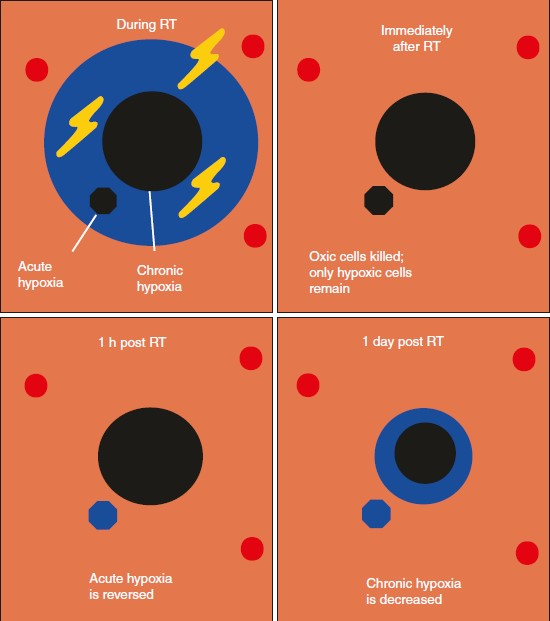
\includegraphics[width=0.5\textwidth]{Imagens/reoxigenacaoAposIrradiacao.jpg}
		}%
		\caption{Escala de tempo da reoxigenação. Após uma dose de radiação suficiente para matar as células normóxicas, mas não as células hipóxicas, apenas as células hipóxicas permanecerão. A reoxigenação ocorre dentro de horas para a hipóxia aguda, mas leva dias para reverter a hipóxia crônica.}
		\label{fig:reoxigenacaoAposIrradiacao}
	\end{figure}

	A \textcolor{DarkTurquoise}{\textbf{\textit{reoxigenação}}} ocorre em duas fases distintas. O \textcolor{MediumOrchid}{\textbf{\textit{componente rápido}}} é observado logo após a irradiação, ocorrendo dentro de algumas horas. Esse rápido aumento nos níveis de oxigênio é atribuído à \textcolor{MediumOrchid}{\textbf{\textit{reoxigenação das regiões hipóxicas agudas do tumor}}}. O \textcolor{MediumOrchid}{\textbf{\textit{componente lento}}} da reoxigenação ocorre ao longo de vários dias e está relacionado à \textcolor{MediumOrchid}{\textbf{\textit{reoxigenação das regiões hipóxicas crônicas do tumor}}}. Essas duas fases refletem a complexa resposta do tumor à irradiação e à reperfusão subsequente.

	A velocidade e a extensão da reoxigenação podem variar entre diferentes tipos de tumores e até mesmo dentro do mesmo tumor. \textcolor{MediumOrchid}{\textbf{\textit{Alguns tumores apresentam uma reoxigenação rápida e completa}}}, onde os níveis de oxigênio são restaurados para valores normais ou quase normais entre as frações de radiação. Isso indica uma \textcolor{MediumOrchid}{\textbf{\textit{eficiente}}} redistribuição do suprimento de oxigênio para as células tumorais. No entanto, \textcolor{MediumOrchid}{\textbf{\textit{outros tumores exibem uma reoxigenação lenta e incompleta}}}, resultando em \textcolor{MediumOrchid}{\textbf{\textit{persistência de hipóxia}}} mesmo após o tratamento fracionado.

	O comportamento da reoxigenação ao longo do curso da radioterapia tem implicações importantes na resposta do tumor ao tratamento. Tumores que se \textcolor{MediumOrchid}{\textbf{\textit{reoxigenam completamente}}} entre as frações de radioterapia mantêm uma \textcolor{MediumOrchid}{\textbf{\textit{radiossensibilidade consistente}}} ao longo do tratamento. Isso significa que a eficácia da radiação permanece alta e as células tumorais continuam sendo afetadas pelas doses subsequentes de radiação. Por outro lado, tumores com \textcolor{MediumOrchid}{\textbf{\textit{reoxigenação incompleta}}} tornam-se cada vez mais hipóxicos a cada fração adicional de radiação. Isso resulta em uma \textcolor{MediumOrchid}{\textbf{\textit{diminuição progressiva da radiossensibilidade}}}, onde as células hipóxicas se tornam menos sensíveis à radiação.

\subsection*{Composição do Tumor em Pacientes}

	A \textcolor{MediumOrchid}{\textbf{\textit{composição heterogênea dos tumores}}} em pacientes é uma característica importante que influencia a resposta ao tratamento. \textcolor{MediumOrchid}{\textbf{\textit{Diferentes populações de células tumorais com mutações genéticas distintas}}} podem \textcolor{MediumOrchid}{\textbf{\textit{coexistir}}} dentro de um tumor, o que pode levar à \textcolor{MediumOrchid}{\textbf{\textit{recorrência}}} após uma resposta completa. Isso é explicado pela presença de \textcolor{DarkTurquoise}{\textbf{\textit{células-tronco tumorais}}}, uma minoria de células dentro do tumor que são responsáveis pela atividade \textcolor{MediumOrchid}{\textbf{\textit{clonogênica}}} e exibem resistência à terapia. Embora a terapia possa eliminar as células não-tronco, as células-tronco tumorais sobreviventes, em pequeno número e clinicamente indetectáveis, têm o potencial de regenerar o tumor.

	Além das células tumorais, os tumores também são compostos por \textcolor{MediumOrchid}{\textbf{\textit{células do hospedeiro}}}, como células vasculares, células estromais\footnote{As células estromais são um tipo de célula do tecido conjuntivo que desempenha um papel fundamentalal no suporte e na manutenção dos órgãos e tecidos do corpo. Elas compõem o estroma, que é o tecido de suporte e estrutural que envolve, sustenta e conecta outros tipos de células em diversos órgãos e tecidos.} e células imunes. Os elementos \textcolor{MediumOrchid}{\textbf{\textit{estromais}}} do tumor incluem fibroblastos associados ao câncer (FACs), células estromais mesenquimais e células endoteliais vasculares. Essas células do estroma estão presentes dentro do tumor e interagem com as células tumorais em uma matriz extracelular complexa, formando o microambiente tumoral.

	A \textcolor{MediumOrchid}{\textbf{\textit{comunicação}}} entre as \textcolor{MediumOrchid}{\textbf{\textit{células tumorais}}} e as \textcolor{MediumOrchid}{\textbf{\textit{células estromais}}} desempenha um papel importante na \textcolor{MediumOrchid}{\textbf{\textit{resistência}}} à quimioterapia e radioterapia. Tanto a quimioterapia citotóxica quanto a radioterapia podem exercer seus efeitos parcialmente por meio de mecanismos mediados pelo sistema imunológico. A \textcolor{MediumOrchid}{\textbf{\textit{imunoterapia}}} e a \textcolor{MediumOrchid}{\textbf{\textit{terapia antiangiogênica}}} têm como \textcolor{MediumOrchid}{\textbf{\textit{alvo}}} as \textcolor{MediumOrchid}{\textbf{\textit{células do hospedeiro}}} em vez das células tumorais. As células tumorais podem expressar moléculas que evitam ou suprimem a resposta imunológica, evitando a ação do sistema imunológico contra elas.

	A \textcolor{MediumOrchid}{\textbf{\textit{hipótese da "vacina in situ"}}} sugere que a \textcolor{MediumOrchid}{\textbf{\textit{radiação}}} ou a \textcolor{MediumOrchid}{\textbf{\textit{quimioterapia}}} podem induzir uma \textcolor{MediumOrchid}{\textbf{\textit{resposta imunológica mais forte}}} por meio dos danos causados às células tumorais. A terapia com íons pesados de carbono tem sido estudada como uma forma de desencadear uma resposta imune aprimorada à radiação. O \textcolor{DarkTurquoise}{\textbf{\textit{``efeito abscopal''}}} refere-se à \textcolor{MediumOrchid}{\textbf{\textit{regressão imunomediada de tumores}}} fora da área irradiada, indicando o \textcolor{MediumOrchid}{\textbf{\textit{impacto sistêmico}}} da radioterapia.

	A \textcolor{MediumOrchid}{\textbf{\textit{combinação de radioterapia e imunoterapia}}}, como o uso de agentes imunoterápicos como ipilimumabe e pembrolizumabe em conjunto com a radioterapia, tem sido explorada para \textcolor{MediumOrchid}{\textbf{\textit{potencializar a resposta imune}}} desencadeada pela radioterapia. Essa abordagem visa atingir tanto as células tumorais quanto as células do sistema imunológico, aumentando assim a eficácia do tratamento e melhorando os resultados para os pacientes.

\section{Cinética de Células e Tecidos}

	A compreensão da cinética celular e tecidual é essencial em radiobiologia e radioterapia porque esses processos têm um impacto significativo na resposta das células e tecidos à radiação. Ao considerar a \textcolor{MediumOrchid}{\textbf{\textit{redistribuição}}} e \textcolor{MediumOrchid}{\textbf{\textit{repopulação}}}, pode-se ajustar as estratégias de tratamento para maximizar a eficácia da radioterapia e minimizar os efeitos colaterais indesejados.

	A \textcolor{DarkTurquoise}{\textbf{\textit{redistribuição celular}}} é importante porque \textcolor{MediumOrchid}{\textbf{\textit{diferentes fases do ciclo celular}}} podem apresentar \textcolor{MediumOrchid}{\textbf{\textit{sensibilidades variadas à radiação}}}. Durante a radioterapia, as células podem ser expostas a diferentes taxas de dose e fracionamento da radiação. Isso pode levar a \textcolor{MediumOrchid}{\textbf{\textit{mudanças na proporção de células em diferentes fases do ciclo celular}}}, afetando a resposta à radiação. Por exemplo, as células em fases mais sensíveis do ciclo celular podem ser deslocadas para fases mais resistentes durante a radioterapia, o que pode reduzir a eficácia do tratamento.

	A \textcolor{DarkTurquoise}{\textbf{\textit{repopulação celular}}} é um fenômeno importante a ser considerado durante o \textcolor{MediumOrchid}{\textbf{\textit{tratamento prolongado}}}. Alguns tecidos têm a capacidade de reabastecer suas populações celulares rapidamente. Durante a radioterapia, a morte de células tumorais ou normais pode levar à \textcolor{MediumOrchid}{\textbf{\textit{ativação de mecanismos de repopulação}}}, resultando no aumento do número de células. Isso pode ter implicações significativas para a eficácia do tratamento, pois uma repopulação mais rápida pode superar os efeitos da radioterapia, reduzindo a resposta terapêutica. Por outro lado, uma repopulação mais lenta pode permitir uma melhor resposta ao tratamento.

\subsection*{Definições}

	\begin{itemize}
		\item \textcolor{DarkTurquoise}{\textbf{G1:}} Fase de intervalo 1, a fase do ciclo celular em que o DNA não está duplicado e a célula se prepara para a síntese do DNA.
		\item \textcolor{DarkTurquoise}{\textbf{S:}} Fase de síntese, a fase do ciclo celular em que o DNA é ativamente replicado ou sintetizado.
		\item \textcolor{DarkTurquoise}{\textbf{G2:}} Fase de intervalo 2, a fase do ciclo celular em que o DNA está completamente duplicado e a célula se prepara para a divisão celular.
		\item \textcolor{DarkTurquoise}{\textbf{M:}} Fase de mitose, a fase do ciclo celular em que os cromossomos se condensam, e o núcleo e a célula se dividem.
		\item \textcolor{DarkTurquoise}{\textbf{$\mathbf{\text{T}_\text{C}}$:}} Tempo do ciclo celular, a duração total de todas as fases do ciclo celular.
		\item \textcolor{DarkTurquoise}{\textbf{$\mathbf{\text{T}_\text{G1}}$:}} Duração da fase G1, o tempo que as células passam na fase G1.
		\item \textcolor{DarkTurquoise}{\textbf{$\mathbf{\text{T}_\text{S}}$:}} Duração da fase S, o tempo que as células passam na fase S.
		\item \textcolor{DarkTurquoise}{\textbf{$\mathbf{\text{T}_\text{G2}}$:}} Duração da fase G2, o tempo que as células passam na fase G2.
		\item \textcolor{DarkTurquoise}{\textbf{$\mathbf{\text{T}_\text{M}}$:}} Duração da fase M, o tempo que as células passam na fase M.
		\item \textcolor{DarkTurquoise}{\textbf{MI:}} Índice mitótico, a porcentagem de células em uma população em mitose em um determinado momento.
		\item \textcolor{DarkTurquoise}{\textbf{LI:}} Índice de marcação, a porcentagem de células que estão incorporando ativamente uma marcação (por exemplo, BrdU) em seu DNA.
		\item \textcolor{DarkTurquoise}{\textbf{$\lambda$:}} Fator de correção da distribuição celular, um parâmetro usado para ajustar a distribuição não uniforme de células nas fases do ciclo celular.
		\item \textcolor{DarkTurquoise}{\textbf{$\mathbf{\text{T}_\text{vol}}$:}} Tempo de duplicação do volume do tumor, o tempo necessário para que um tumor dobre de tamanho.
		\item \textcolor{DarkTurquoise}{\textbf{$\mathbf{\text{T}_\text{d}}$:}} Tempo de duplicação do diâmetro do tumor, o tempo necessário para que o diâmetro de um tumor dobre de tamanho.
		\item \textcolor{DarkTurquoise}{\textbf{$\mathbf{\text{T}_\text{pot}}$:}} Tempo de duplicação potencial do tumor, uma medida do tempo necessário para que toda a população de células do tumor dobre de tamanho.
		\item \textcolor{DarkTurquoise}{\textbf{GF:}} Fração de crescimento, a proporção de células proliferativas em um tumor.
		\item \textcolor{DarkTurquoise}{\textbf{CLF ($\phi$):}} Fator de perda celular, um fator que leva em consideração a perda de células por meio de fatores como apoptose, necrose ou eliminação.
	\end{itemize}

\subsection*{Ciclo Celular}

	A biologia molecular do \textcolor{DarkTurquoise}{\textbf{\textit{ciclo celular}}} (\ref{fig:cicloCelular}) é essencial para entender a regulação precisa da divisão celular e como ela pode ser afetada em condições patológicas, como o câncer. O ciclo celular é controlado por \textcolor{MediumOrchid}{\textbf{\textit{checkpoints}}}, onde a \textcolor{MediumOrchid}{\textbf{\textit{progressão é monitorada}}} para garantir uma divisão celular correta.

	\begin{figure}[h]
		\centering
		\fcolorbox{DarkTurquoise}{white}{%
			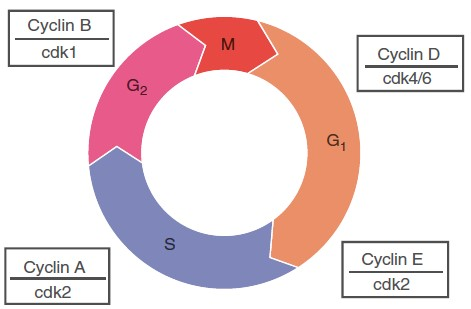
\includegraphics[width=0.5\textwidth]{Imagens/cicloCelular.jpg}
		}%
		\caption{Ciclo celular. O ciclo celular é regulado por pontos de checagem que são controlados por complexos Cdk-Ciclina, os quais são sensíveis a vários sinais dentro da célula.}
		\label{fig:cicloCelular}
	\end{figure}

	Em cada \textcolor{MediumOrchid}{\textbf{\textit{checkpoint}}}, a \textcolor{MediumOrchid}{\textbf{\textit{atividade}}} do ciclo celular é \textcolor{MediumOrchid}{\textbf{\textit{regulada}}} por complexos formados por \textcolor{MediumOrchid}{\textbf{\textit{ciclinas e quinases dependentes de ciclina}}} (Cdks), bem como seus \textcolor{MediumOrchid}{\textbf{\textit{inibidores}}}. As ciclinas são proteínas que se ligam às Cdks e ativam sua atividade, enquanto os inibidores atuam como reguladores negativos, impedindo a atividade das Cdks quando necessário.

	O \textcolor{DarkTurquoise}{\textbf{\textit{checkpoint G1/S}}} é um dos principais pontos de controle no ciclo celular. Ele é regulado por complexos de ciclina D e Cdk4/6, que desempenham um papel crucial na transição da fase G1 para a fase S. A ativação da ciclina D é induzida por sinais mitogênicos, que estimulam a proliferação celular. O complexo ciclina D/Cdk4/6 fosforila e inativa a proteína supressora de tumor retinoblastoma (Rb), liberando o fator de transcrição E2F. E2F, por sua vez, ativa a transcrição de genes envolvidos na síntese de DNA, incluindo as ciclinas E e A, essenciais para a progressão do ciclo celular.

	A \textcolor{DarkTurquoise}{\textbf{\textit{p53}}} é um importante regulador do ciclo celular que desempenha um papel crítico na integridade do genoma. Em \textcolor{MediumOrchid}{\textbf{\textit{resposta a danos no DNA}}} ou estresse celular, o \textcolor{MediumOrchid}{\textbf{\textit{p53 é ativado}}} e \textcolor{MediumOrchid}{\textbf{\textit{induz a expressão da p21}}}, uma inibidora das Cdks. Isso \textcolor{MediumOrchid}{\textbf{\textit{bloqueia a transição do ciclo celular na fase G1/S}}}, permitindo a reparação do DNA danificado antes da replicação.

	\textcolor{MediumOrchid}{\textbf{\textit{Alterações genéticas}}} que afetam diretamente proteínas-chave envolvidas na regulação do ciclo celular, como Rb e p53, são frequentemente observadas em tumores. Mutações ou desregulação dessas proteínas podem levar a uma \textcolor{MediumOrchid}{\textbf{\textit{entrada descontrolada na fase S}}} e promover a \textcolor{MediumOrchid}{\textbf{\textit{proliferação descontrolada das células tumorais}}}.

	A transição do ciclo celular da fase G2 para a fase M é regulada pelo complexo ciclina B/Cdk1. A ativação desse complexo promove a fosforilação da histona H1 e das lamínas nucleares, levando à condensação dos cromossomos e dissolução da membrana nuclear em preparação para a mitose.

	É importante destacar que o \textcolor{MediumOrchid}{\textbf{\textit{checkpoint G2/M}}} é geralmente \textcolor{MediumOrchid}{\textbf{\textit{mantido}}} na maioria dos cânceres, o que \textcolor{MediumOrchid}{\textbf{\textit{impede a entrada na fase M}}} de células com danos no DNA ou outros problemas celulares.

\subsection*{Parâmetros do Ciclo Celular}

	Nas células de mamíferos os tempos \textcolor{MediumOrchid}{\textbf{$\text{T}_\text{S}$}}, \textcolor{MediumOrchid}{\textbf{$\text{T}_\text{G2}$}} e \textcolor{MediumOrchid}{\textbf{$\text{T}_\text{M}$}} apresentam pouca variação:

	\begin{itemize}
		\item \textcolor{DarkTurquoise}{\textbf{$\text{T}_\text{S}$}} 6-8 horas.
		\item \textcolor{DarkTurquoise}{\textbf{$\text{T}_\text{G2}$}} 3-4 horas.
		\item \textcolor{DarkTurquoise}{\textbf{$\text{T}_\text{M}$}} 1 hora.
		\end{itemize}
		
		No entanto, a duração da fase G1, \textcolor{MediumOrchid}{\textbf{$\text{T}_\text{G1}$}},  pode variar significativamente, dependendo do tipo de célula:
		
		\begin{itemize}
		\item Células CHO de hamster têm um \textcolor{DarkTurquoise}{\textbf{$\text{T}_\text{G1}$}} de 1 hora.
		\item Células tumorais humanas HeLa têm um \textcolor{DarkTurquoise}{\textbf{$\text{T}_\text{G1}$}} de 11 horas.
		\item Células tumorais humanas de crescimento lento podem ter um \textcolor{DarkTurquoise}{\textbf{$\text{T}_\text{G1}$}} de vários dias.
	\end{itemize}

\subsection*{Cinética de Crescimento de Tumores Clínicos}

	A cinética de crescimento dos tumores clínicos é uma área importante de estudo que busca compreender a \textcolor{MediumOrchid}{\textbf{\textit{taxa de crescimento e a resposta dos tumores ao tratamento}}}. Algumas características cinéticas dos tumores incluem o tempo de ciclo celular ($TC$), o tempo de duplicação potencial ($T_{\text{pot}}$), o tempo de duplicação do volume ($T_{\text{vol}}$) e o tempo de duplicação do diâmetro ($T_{\text{d}}$).

	Um \textcolor{MediumOrchid}{\textbf{\textit{tumor "médio"}}} humano é estimado ter um $TC$ de 2 dias e um $T_{\text{pot}}$ de 5 dias. Isso significa que as células do tumor levam cerca de 2 dias para completar um ciclo de crescimento e o tumor tem o potencial de dobrar de tamanho em aproximadamente 5 dias. Com um fator de perda celular ($\phi$) de 75\%, que representa a fração de células que são perdidas por morte celular ou outros mecanismos, o $T_{\text{vol}}$ é estimado em 20 dias e o $T_{\text{d}}$ é estimado em 60 dias. É importante ressaltar que esses valores podem variar amplamente entre pacientes e até mesmo entre diferentes metástases no mesmo paciente. Cada tumor tem suas próprias características e pode apresentar um $TC$, $T_{\text{pot}}$ e $\phi$ diferentes. Conforme os tumores crescem, eles podem se tornar mais \textcolor{MediumOrchid}{\textbf{\textit{necróticos}}}, o que significa que uma maior porção do tumor é composta por tecido morto. Isso aumenta o valor de $\phi$, levando a um aumento no tempo de duplicação do volume e do diâmetro.

	A \textcolor{DarkTurquoise}{\textbf{\textit{repopulação acelerada}}} é um fenômeno observado em alguns tipos de câncer, como \textcolor{MediumOrchid}{\textbf{\textit{cânceres de células escamosas da cabeça e do pescoço e do colo do útero}}} (\ref{fig:repopulacaoAcelerada}). Nesse fenômeno, o \textcolor{MediumOrchid}{\textbf{\textit{tratamento citotóxico prolongado}}}\footnote{Um tratamento citotóxico é um tipo de terapia que utiliza substâncias ou agentes citotóxicos (quimioterápicos) para destruir ou inibir o crescimento de células em divisão. Essa abordagem é frequentemente usada no tratamento de doenças caracterizadas por crescimento celular descontrolado, como o câncer.} estimula as células tumorais a se dividirem mais rapidamente, resultando em um aumento na taxa de crescimento do tumor.

	\begin{figure}[h]
		\centering
		\fcolorbox{DarkTurquoise}{white}{%
			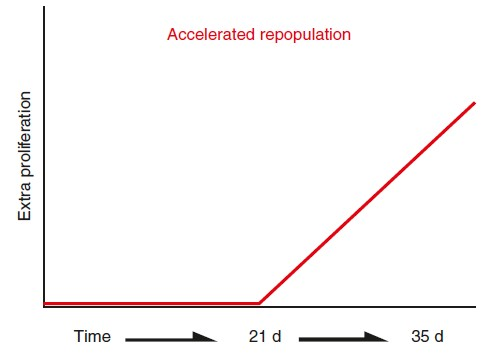
\includegraphics[width=0.5\textwidth]{Imagens/repopulacaoAcelerada.jpg}
		}%
		\caption{Uma vez iniciado o tratamento, certos tumores podem passar por um processo conhecido como repopulação acelerada, que se inicia em um tempo específico denominado "tempo de início" ou "kickoff time".}
		\label{fig:repopulacaoAcelerada}
	\end{figure}

	A repopulação acelerada é caracterizada por um "tempo de início" ($T_k$), que é um atraso de aproximadamente 21 a 28 dias desde o início do tratamento até o início da repopulação acelerada. Uma vez que a repopulação acelerada começa, o $T_d$ se aproxima do $T_{\text{pot}}$, o que significa que o tumor passa a crescer mais rapidamente do que o usual.

\subsection*{Repopulação Acelerada e Dose Efetiva}

	A repopulação acelerada é um fenômeno que ocorre durante o \textcolor{MediumOrchid}{\textbf{\textit{tratamento prolongado}}} de cânceres e resulta em um \textcolor{MediumOrchid}{\textbf{\textit{aumento na taxa de crescimento}}} do tumor. Para contrabalançar a repopulação acelerada, uma \textcolor{MediumOrchid}{\textbf{\textit{dose adicional de radiação}}}, conhecida como $D_{\text{prolif}}$, deve ser administrada.

	O valor de $D_{\text{prolif}}$ varia de 0.4 Gy a 0.8 Gy por dia para células tumorais de cabeça e pescoço, pulmão e sistema nervoso central (SNC). Essa dose diária adicional é necessária para combater o crescimento acelerado das células tumorais durante o tratamento prolongado.

	É importante ressaltar que \textcolor{MediumOrchid}{\textbf{\textit{o tratamento prolongado}}}, juntamente com a repopulação acelerada, também \textcolor{MediumOrchid}{\textbf{\textit{aumenta a sobrevivência das células normais em proliferação}}}, como pele e mucosa. Esses tecidos normais têm a capacidade de se regenerar e se repopular durante o tratamento, resultando em uma \textcolor{MediumOrchid}{\textbf{\textit{melhor recuperação}}} e \textcolor{MediumOrchid}{\textbf{\textit{menor toxicidade aguda}}}.

	No entanto, é necessário ter cuidado ao administrar doses adicionais durante o tratamento prolongado, pois isso pode \textcolor{MediumOrchid}{\textbf{\textit{aumentar o risco de toxicidade tardia em tecidos normais e potencialmente afetar a qualidade de vida dos pacientes}}}. A administração de doses extras deve ser cuidadosamente planejada e equilibrada com os riscos e benefícios potenciais.

	Essa é uma das razões pelas quais a terapia com intervalos de tratamento, que envolve pausas intencionais no tratamento, tem diminuído em popularidade. A administração contínua de tratamento, sem pausas prolongadas, ajuda a minimizar o risco de repopulação acelerada, mas também requer uma consideração cuidadosa da dose total e dos efeitos nos tecidos normais. Os esquemas de tratamento são projetados levando em conta esses fatores para equilibrar a eficácia do tratamento com a toxicidade potencial.

\subsection*{Sincronização do Ciclo Celular}

	A \textcolor{MediumOrchid}{\textbf{\textit{sincronização do ciclo celular}}} é uma técnica utilizada em estudos para investigar e\textcolor{MediumOrchid}{\textbf{\textit{feitos dependentes do ciclo celular}}}, como a replicação do DNA, a expressão gênica e a resposta a tratamentos específicos. Existem várias técnicas que podem ser empregadas para sincronizar as células em uma fase específica do ciclo celular. São elas:

	\begin{itemize}
	\item \textcolor{DarkTurquoise}{\textbf{Colheita mitótica (shakeoff):}} Nesse método, as células são cultivadas em uma monocamada aderente a um recipiente. Durante a mitose, as células perdem temporariamente a adesão e podem ser fisicamente desalojadas (shakeoff) para serem utilizadas em experimentos. Isso permite obter uma população enriquecida em células em mitose.

	\item \textcolor{DarkTurquoise}{\textbf{Hidroxiureia (HU):}} A HU é uma droga que seletivamente mata as células na fase S do ciclo celular. Ao serem incubadas com HU, as células se acumulam no checkpoint G1-S, aguardando a entrada na fase S do ciclo celular. Posteriormente, a remoção da HU permite que as células prossigam para a fase S.

	\item \textcolor{DarkTurquoise}{\textbf{Outras drogas:}} Diversas drogas podem ser utilizadas para sincronizar as células em uma fase específica do ciclo celular, dependendo do objetivo do estudo. Por exemplo, drogas como inibidores de quinases específicas podem bloquear uma fase específica do ciclo celular, permitindo a análise de eventos relacionados a essa fase.
	\end{itemize}

\subsection*{Ciclo Celular e Radiossensibilidade}

	O ciclo celular desempenha um papel crucial na resposta das células à radioterapia. A sensibilidade das células tumorais à radiação varia ao longo das diferentes fases do ciclo celular, o que tem implicações na eficácia do tratamento. Alguns pontos importantes relacionados ao ciclo celular e à radiossensibilidade são os seguintes:

	\begin{itemize}
		\item \textcolor{DarkTurquoise}{\textbf{Sensibilidade geral (D0):}} As células são mais \textcolor{MediumOrchid}{\textbf{\textit{sensíveis}}} à radioterapia na fase \textcolor{MediumOrchid}{\textbf{\textit{G2/M}}}do ciclo celular. Nessa fase, as células estão prestes a se dividir, e o tempo disponível para reparar os danos no DNA antes da divisão é limitado. Isso pode levar a uma maior probabilidade de catástrofe mitótica, resultando em morte celular.

		\item \textcolor{DarkTurquoise}{\textbf{Reparação por recombinação homóloga:}} Durante a \textcolor{MediumOrchid}{\textbf{\textit{fase S tardia}}}, após a replicação do DNA, a reparação por recombinação homóloga é mais ativa. Isso pode aumentar a capacidade das células de reparar danos no DNA e, consequentemente, reduzir sua sensibilidade à radiação \textcolor{MediumOrchid}{\textbf{\textit{(mais radiorresistente)}}}.

		\item \textcolor{DarkTurquoise}{\textbf{Tamanho do ombro (Dq):}} A curva de sobrevivência após a exposição à radiação apresenta um ombro, que indica o \textcolor{MediumOrchid}{\textbf{\textit{reparo dos danos causados pela radiação}}}. O tamanho do ombro varia ao longo das diferentes fases do ciclo celular. É \textcolor{MediumOrchid}{\textbf{\textit{mínimo na fase G2/M}}}, \textcolor{MediumOrchid}{\textbf{\textit{moderado na fase G1 até a fase inicial da S}}} e \textcolor{MediumOrchid}{\textbf{\textit{significativo na fase S tardia}}}.

		\item \textcolor{DarkTurquoise}{\textbf{Dependência de oxigênio (OER):}} O \textcolor{MediumOrchid}{\textbf{\textit{OER}}} é mais \textcolor{MediumOrchid}{\textbf{\textit{alto na fase S}}} do ciclo celular. Isso ocorre porque \textcolor{MediumOrchid}{\textbf{\textit{a reparação do DNA é mais ativa em condições de hipóxia}}}, quando o oxigênio é escasso. No entanto, é importante notar que o oxigênio também dificulta a reparação dos danos no DNA, resultando em uma dependência complexa do oxigênio no efeito da radiação.

		\item \textcolor{DarkTurquoise}{\textbf{Radiação de alto LET:}} A dependência do ciclo celular na sensibilidade à radiação ainda existe para radiação de alto LET, mas é reduzida em comparação com a radiação de baixo LET. A radiação de alto LET causa danos mais complexos no DNA, que podem ser mais difíceis de reparar, independentemente da fase do ciclo celular.
	\end{itemize}

\subsection*{Radioterapia Fracionada e Rearranjo}

	Na \textcolor{MediumOrchid}{\textbf{\textit{radioterapia fracionada}}}, o tratamento é administrado em várias frações ao longo de um período de tempo. \textcolor{MediumOrchid}{\textbf{\textit{Esse regime de tratamento permite que as células tumorais passem por um processo chamado rearranjo entre as frações}}}. O \textcolor{DarkTurquoise}{\textbf{\textit{rearranjo}}} é o mecanismo pelo qual as células tumorais \textcolor{MediumOrchid}{\textbf{\textit{redistribuem-se}}} entre as fases ou partes do ciclo celular mais sensíveis à radiação.

	Uma característica importante do rearranjo é que as \textcolor{MediumOrchid}{\textbf{\textit{células tumorais na fase S}}}, que são conhecidas por serem radiorresistentes, têm a oportunidade de se \textcolor{MediumOrchid}{\textbf{\textit{redistribuir para fases mais sensíveis à radiação}}}, como G1 ou G2/M. Isso ocorre porque, durante o intervalo entre as frações, as células na fase S continuam seu ciclo celular e eventualmente avançam para outras fases. À medida que as células progridem pelo ciclo celular, elas se tornam mais sensíveis à radiação.

	Esse processo de rearranjo é benéfico na radioterapia fracionada, pois \textcolor{MediumOrchid}{\textbf{\textit{aumenta a eficácia do tratamento}}}. As células tumorais radiorresistentes presentes na fase S durante uma fração podem ser redistribuídas para fases mais sensíveis à radiação antes da próxima fração, tornando-as mais suscetíveis à ação da radiação. Isso melhora a razão terapêutica da radioterapia fracionada, permitindo que as células sejam eliminadas mais efetivamente.

	Além disso, em certos cenários de \textcolor{MediumOrchid}{\textbf{\textit{baixa taxa de dose (LDR)}}}, as células tumorais podem \textcolor{MediumOrchid}{\textbf{\textit{progredir pelo ciclo celular}}} e \textcolor{MediumOrchid}{\textbf{\textit{acumular-se na fase G2}}}. \textcolor{MediumOrchid}{\textbf{\textit{A fase G2 é mais sensível à radiação}}}, o que significa que uma dose mais baixa de radiação pode resultar em uma maior resposta terapêutica. Esse fenômeno é conhecido como \textcolor{MediumOrchid}{\textbf{\textit{efeito inverso da taxa de dose}}}, onde a sobrevivência celular diminui com taxas de dose mais baixas em vez de aumentar.

\section{Efeitos de Dose e Fracionamento}

\subsection*{Definições de Fracionamento}

	As definições de fracionamento são importantes na radioterapia para descrever diferentes esquemas de tratamento que envolvem a administração da radiação em várias frações ao longo do tempo. Aqui estão algumas definições comuns de fracionamento:

	\begin{itemize}
		\item \textcolor{DarkTurquoise}{\textbf{Fracionamento Padrão:}} É o esquema de tratamento mais comum, em que a radioterapia é administrada uma vez ao dia, cinco dias por semana, com uma dose máxima de 2 Gy por fração. Esse regime é usado para equilibrar a eficácia do tratamento com a minimização dos efeitos colaterais nos tecidos normais.

		\item \textcolor{DarkTurquoise}{\textbf{Fracionamento com Intervalos:}} Nesse esquema, pausas intencionais são planejadas durante o tratamento, geralmente por motivos clínicos, como permitir a recuperação dos tecidos normais. Esses intervalos podem ser úteis para minimizar a toxicidade tardia.

		\item \textcolor{DarkTurquoise}{\textbf{Fracionamento Alterado:}} Refere-se a qualquer esquema de fracionamento que difere do fracionamento padrão. Pode envolver a variação do número de frações, tamanhos de fração ou frequência de tratamento para melhor atender às necessidades do paciente.

		\item \textcolor{DarkTurquoise}{\textbf{Fracionamento Acelerado:}} Envolve a administração de uma dose total maior de radiação por unidade de tempo em comparação com o fracionamento padrão. Subtipos incluem fracionamento acelerado puro, hipofracionamento acelerado e hiperfracionamento acelerado, dependendo do tamanho da fração e do número de frações por semana.

		\item \textcolor{DarkTurquoise}{\textbf{Hipofracionamento:}} Envolve o aumento do tamanho da fração (dose recebida por fração), com ou sem diminuição do número de frações por semana. Pode ser utilizado em certos tipos de tumores para um tratamento mais conveniente ou para explorar efeitos biológicos favoráveis.

		\item \textcolor{DarkTurquoise}{\textbf{Radioterapia Estereotáxica (SRS/SBRT/SABR):}} É uma forma especializada de fracionamento em que a radioterapia é entregue com técnicas de localização precisa, geralmente em cinco frações ou menos. É usado para tratar lesões pequenas e bem definidas com alta precisão.

		\item \textcolor{DarkTurquoise}{\textbf{Radioterapia Estereotáxica Fracionada (FSRT):}} Similar à radioterapia estereotáxica, mas com mais de cinco frações. Também envolve técnicas estereotáxicas para entregar doses precisas de radiação em volumes de tratamento complexos.

		\item \textcolor{DarkTurquoise}{\textbf{Hiperfracionamento:}} Envolve a diminuição do tamanho da fração (menor dose por fração) com mais de uma fração por dia (BID - duas vezes ao dia - ou TID - três vezes ao dia). É usado em situações específicas para melhorar a eficácia do tratamento.

		\item \textcolor{DarkTurquoise}{\textbf{Boost Concomitante (CB):}} Envolve a administração de duas frações por dia, sendo uma fração para um campo grande e a outra para um volume de boost. É usado para fornecer uma dose mais alta a um volume específico enquanto se administra a radioterapia no campo geral.

		\item \textcolor{DarkTurquoise}{\textbf{Boost Integrado Simultâneo (SIB):}} Envolve a administração de uma fração por dia, com uma dose mais alta para um volume de boost e uma dose mais baixa para o campo geral. É usado para fornecer um boost de dose focalizado durante a radioterapia padrão.
	\end{itemize}

\subsection*{Modelo Linear-Quadrático (LQ, Alfa-Beta)}

	O modelo linear-quadrático (LQ) é um modelo matemático usado na radiobiologia para descrever a resposta das células e tecidos à radiação. Ele foi desenvolvido com base em observações experimentais que mostraram que os danos ao DNA causados pela radiação apresentam uma relação linear-quadrática com a dose (\ref{fig:modeloLinearQuadratico}).

	\begin{figure}[h]
		\centering
		\fcolorbox{DarkTurquoise}{white}{%
			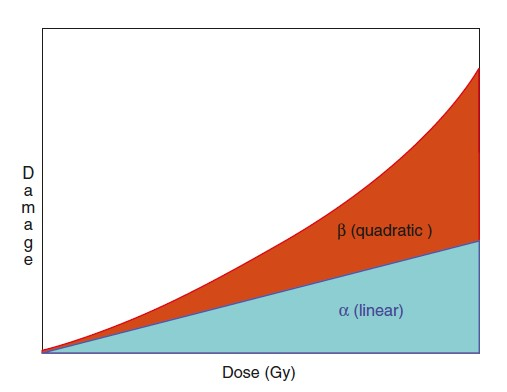
\includegraphics[width=0.5\textwidth]{Imagens/modeloLinearQuadratico.jpg}
		}%
		\caption{A curva de danos ao DNA linear-quadrático representa o dano total ao DNA como a soma do dano "linear", que não depende do tamanho da fração, e do dano "quadrático", que depende do tamanho da fração.}
		\label{fig:modeloLinearQuadratico}
	\end{figure}

	A fórmula do modelo LQ é dada por: Aberrações letais do DNA = $\alpha D + \beta D^2$, onde $\alpha$ e $\beta$ são parâmetros específicos do tecido que representam os danos letais ao DNA.

	No modelo LQ, \textcolor{MediumOrchid}{\textbf{\textit{o efeito da radiação na mortalidade celular é calculado com base nessas aberrações letais do DNA}}}. O termo $\alpha D$ representa os danos irreparáveis ao DNA causados por um único impacto de radiação, enquanto o termo $\beta D^2$ representa os danos reparáveis ao DNA acumulados ao longo de múltiplos impactos.

	A fração de sobrevivência (SF) pode ser calculada usando a equação $\text{SF}_D = e^{-({\alpha D + \beta D^2})}$, onde $D$ é a dose total de radiação.

	A razão $\alpha/\beta$ é um parâmetro importante no modelo LQ, pois indica \textcolor{MediumOrchid}{\textbf{\textit{a dose em que as mortes causadas pelos danos irreparáveis ($\alpha$) e pelos danos reparáveis ($\beta$) são iguais}}}. Essa razão é uma medida da \textcolor{MediumOrchid}{\textbf{\textit{sensibilidade}}} do tecido à radioterapia.

	Tecidos com uma \textcolor{MediumOrchid}{\textbf{\textit{baixa razão $\alpha/\beta$}}}, ou seja, ``alta reparação'', são relativamente \textcolor{MediumOrchid}{\textbf{\textit{resistentes a pequenos tamanhos de fração}}} (doses pequenas por fração), o que significa que eles se recuperam bem entre as frações de radioterapia. No entanto, eles são relativamente \textcolor{MediumOrchid}{\textbf{\textit{sensíveis a grandes tamanhos de fração}}} (altas doses por fração), pois têm menos capacidade de reparação entre as doses altas.

	Por outro lado, tecidos com uma \textcolor{MediumOrchid}{\textbf{\textit{alta razão $\alpha/\beta$}}}, ou seja, ``baixa reparação'', são relativamente \textcolor{MediumOrchid}{\textbf{\textit{sensíveis a pequenos tamanhos de fração}}} (baixa dose por fração), mas têm uma \textcolor{MediumOrchid}{\textbf{\textit{maior capacidade de reparação entre as doses altas}}}, tornando-os mais \textcolor{MediumOrchid}{\textbf{\textit{resistentes}}} a grandes tamanhos de fração.

\subsection*{Razão Alfa-Beta para Tecidos}

	A razão $\alpha/\beta$ é um parâmetro importante na radiobiologia que descreve a resposta de um tecido ou tumor à radiação. Alguns exemplos das razões $\alpha/\beta$ associadas a diferentes tecidos e tumores são:

	\begin{itemize}
		\item \textcolor{DarkTurquoise}{\textbf{Tecidos de reação aguda:}} Esses tecidos, como pele, intestino delgado e mucosa oral, são conhecidos por ter uma \textcolor{MediumOrchid}{\textbf{\textit{resposta rápida à radiação}}} e podem apresentar reações agudas, como eritema, mucosite e diarreia. Eles geralmente têm uma \textcolor{MediumOrchid}{\textbf{\textit{razão $\alpha/\beta \approx 10$}}} .

		\item \textcolor{DarkTurquoise}{\textbf{Tecidos de reação tardia:}} Esses tecidos, como pulmão, fígado e rins, são mais propensos a desenvolver reações tardias à radiação, como fibrose e disfunção. Eles tendem a ter uma razão \textcolor{MediumOrchid}{\textbf{\textit{$\alpha/\beta \lessapprox 3$}}}.

		\item \textcolor{DarkTurquoise}{\textbf{Tecidos do sistema nervoso central (SNC):}} O cérebro e a medula espinhal são tecidos do SNC e acredita-se que esses tecidos tenham uma razão $1 \lessapprox \alpha/\beta \lessapprox 2$.

		\item \textcolor{DarkTurquoise}{\textbf{Tumores:}} A maioria dos tumores é geralmente mais resistente à radiação do que os tecidos normais. Eles tendem a ter uma razão \textcolor{MediumOrchid}{\textbf{\textit{$\alpha/\beta \geq 10 $}}}. Isso significa que eles respondem melhor a doses maiores por fração, como na radioterapia hipofracionada ou fracionamento acelerado.

		\item \textcolor{DarkTurquoise}{\textbf{Tumores de mama e próstata:}} Alguns tumores com tumores com baixa razão $\alpha/\beta$ tem uma razão $1.5 \lessapprox \alpha/\beta \lessapprox 4$. Os \textcolor{MediumOrchid}{\textbf{\textit{tumores de mama e próstata são considerados exemplos clássicos de tumores com baixa razão $\alpha/\beta$}}}. Isso significa que eles são mais sensíveis a doses menores por fração, como na radioterapia com fracionamento padrão.
		
	\end{itemize}

\subsection*{Modelo Alfa-Beta e Fracionamento de Dose}

O modelo alfa-beta desempenha um papel importante no fracionamento da dose na radioterapia. Algumas considerações quanto ao seu papel são:

	\begin{itemize}
		\item \textcolor{DarkTurquoise}{\textbf{Razão alfa-beta mais alta em tumores:}} O modelo alfa-beta sugere que os tumores têm uma razão alfa-beta mais alta em comparação aos tecidos normais. Isso significa que \textcolor{MediumOrchid}{\textbf{\textit{os tumores são relativamente mais sensíveis a doses maiores por fração}}} em comparação aos tecidos normais (\ref{fig:fracionamentoEMorteCelular}).
		
		\begin{figure}[h]
			\centering
			\fcolorbox{DarkTurquoise}{white}{%
				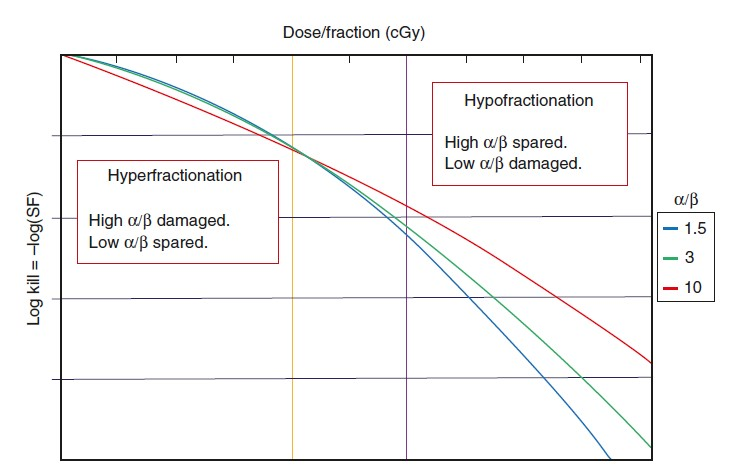
\includegraphics[width=0.5\textwidth]{Imagens/fracionamentoEMorteCelular.jpg}
			}%
			\caption{Tamanho da fração e mortalidade relativa: Tamanhos de fração menores são comparativamente mais eficazes em causar a morte celular em tecidos com uma alta razão alfa/beta. Por outro lado, tamanhos de fração maiores são relativamente mais eficazes na morte de tecidos com uma baixa razão alfa/beta.}
			\label{fig:fracionamentoEMorteCelular}
		\end{figure}

		\item \textcolor{DarkTurquoise}{\textbf{Poupar tecidos normais:}} O fracionamento da dose permite que \textcolor{MediumOrchid}{\textbf{\textit{tecidos normais com uma razão alfa-beta mais baixa sejam poupados de danos excessivos}}}. Ao administrar doses menores por fração, os tecidos normais têm mais tempo para reparar os danos causados pela radiação, resultando em menor toxicidade aguda e tardia.

		\item \textcolor{DarkTurquoise}{\textbf{Sensibilidade aumentada de tecidos de resposta tardia:}} Tecidos de resposta tardia, como o sistema nervoso central, têm uma baixa razão alfa-beta. Isso significa que eles são \textcolor{MediumOrchid}{\textbf{\textit{mais sensíveis a doses menores por fração}}}. Portanto, para esses tecidos, é necessário ter precaução ao selecionar tamanhos de fração para evitar efeitos colaterais graves.

		\item \textcolor{DarkTurquoise}{\textbf{Benefícios limitados para tumores com baixa relação alfa-beta:}} Tumores com uma \textcolor{MediumOrchid}{\textbf{\textit{razão alfa-beta baixa}}}, como alguns tumores de mama e próstata, podem \textcolor{MediumOrchid}{\textbf{\textit{não experimentar benefícios significativos do fracionamento da dose}}}. Isso ocorre porque esses tumores respondem de maneira semelhante a doses maiores ou menores por fração, e doses menores por fração podem prolongar desnecessariamente a duração do tratamento.
	\end{itemize}

\subsection*{BED e o Modelo Alfa-Beta}

	O modelo alfa-beta, baseado no conceito linear-quadrático, é uma ferramenta na radioterapia que \textcolor{MediumOrchid}{\textbf{\textit{permite o cálculo das doses eficazes para diferentes tamanhos de fração}}}. Isso torna o modelo altamente prático na prática clínica. Uma medida importante nesse contexto é a \textcolor{MediumOrchid}{\textbf{\textit{dose biologicamente eficaz (BED)}}}, que é uma dose extrapolada ao longo de um número de frações. Em contraste, a Dose Padrão Nominal (NSD) representa uma dose equivalente em uma única fração.

	Para um tratamento com $n$ frações de dose $d$ por fração, a equação para determinar a $\text{BED}_{\alpha/\beta}$ é dada por:

	\begin{equation}
		\text{BED}_{\alpha/\beta} = n \times d \times \left(1 + \frac{d}{\alpha/\beta}\right)
	\end{equation}

	É essencial destacar que a \textcolor{MediumOrchid}{\textbf{\textit{BED é sempre maior do que a dose física ($n \times d$)}}}.
	
	\

	\begin{tcolorbox}[width=\textwidth, colback={white}, colbacktitle={DarkTurquoise!50!white}, title={$\bigstar$ \LobsterTwo{Exemplo: Cálculo do BED} $\bigstar $}, coltitle={CarnationPink}, colframe={DarkTurquoise}, fonttitle=\rmfamily\bfseries\Large, breakable]

		\begin{itemize}[label=\textcolor{CarnationPink}{$\blacktriangleright$}]
			\item Suponha que desejamos limitar a dose máxima na medula espinhal, com um valor \textcolor{MediumOrchid}{\textbf{\textit{$\alpha/\beta = 2$}}}, a uma \textcolor{MediumOrchid}{\textbf{\textit{$\text{BED}_2$ máxima de 98 Gy}}}. 
			\item Se estivermos usando frações diárias de \textcolor{MediumOrchid}{\textbf{\textit{3 Gy}}}, calculamos a $\text{BED}_2$ para cada fração (\textcolor{MediumOrchid}{\textbf{\textit{$\text{BED}_2(3 \text{ Gy}) = 3 \times 2.5 = 7.5 \text{ Gy}_2$}}}). 
			\item Dividindo 98 $\text{ Gy}_2$ por 7.5, encontramos aproximadamente \textcolor{MediumOrchid}{\textbf{\textit{13.07 frações}}}.
			\item Portanto, a dose máxima deve ser \textcolor{MediumOrchid}{\textbf{\textit{$13 \times 3 \text{ Gy} = 39 \text{ Gy}$}}}.
		\end{itemize}
	\end{tcolorbox}
	
	\
	
	Outro parâmetro relevante é a \textcolor{MediumOrchid}{\textbf{\textit{dose equivalente em frações de 2 Gy/dia ($\text{EQD}_{\alpha/\beta, 2}$)}}}. Esse valor permite a combinação de cursos de tratamento parciais que foram administrados com diferentes tamanhos de fração. A equação para calcular a $\text{EQD}_{\alpha/\beta, 2}$ é:

	\begin{equation}
		\text{EQD}_{\alpha/\beta, 2} = n \times d \times \left(\frac{\alpha/\beta + d}{\alpha/\beta + 2}\right)
	\end{equation}

	\begin{tcolorbox}[width=\textwidth, colback={white}, colbacktitle={DarkTurquoise!50!white}, title={$\bigstar$ \LobsterTwo{Exemplo: Cálculo do EQD\textsubscript{2}} $\bigstar$}, coltitle={CarnationPink}, colframe={DarkTurquoise}, fonttitle=\rmfamily\bfseries\Large, breakable]

		\begin{itemize}[label=\textcolor{CarnationPink}{$\blacktriangleright$}]
			\item Suponha que estamos tratando um câncer de pulmão com uma dose total de \textcolor{MediumOrchid}{\textbf{\textit{60 Gy em frações de 2 Gy/dia}}}, mas as primeiras cinco frações foram administradas com \textcolor{MediumOrchid}{\textbf{\textit{3 Gy}}} devido à síndrome da veia cava superior.
			\item Assumindo um valor \textcolor{MediumOrchid}{\textbf{\textit{$\alpha/\beta = 3$}}}, podemos calcular a dose adicional necessária em frações de \textcolor{MediumOrchid}{\textbf{\textit{2 Gy/dia}}}. 
			\item Multiplicando \textcolor{MediumOrchid}{\textbf{\textit{3 Gy por 5}}}, obtemos \textcolor{MediumOrchid}{\textbf{\textit{15 Gy}}}. 
			\item Ao aplicar a equação \textcolor{MediumOrchid}{\textbf{\textit{$\text{EQD}_{3,2} = 15 \times \frac{6}{5}$}}}, encontramos o equivalente de \textcolor{MediumOrchid}{\textbf{\textit{18 Gy}}}.
			\item Portanto, ainda precisamos administrar \textcolor{MediumOrchid}{\textbf{\textit{$60 \text{ Gy} - 18 \text{ Gy} = 42 \text{ Gy}$}}} em frações de \textcolor{MediumOrchid}{\textbf{\textit{2 Gy/dia}}}.
		\end{itemize}
	\end{tcolorbox}

\subsection*{Fatores de Correção do Modelo Alfa-Beta}

	O modelo alfa-beta considera diversos fatores de correção para ajustar os cálculos e levar em conta condições específicas de tratamento. Um desses fatores é o\textcolor{DarkTurquoise}{\textbf{\textit{ fator de correção H de Thames}}}, que é aplicado a \textcolor{MediumOrchid}{\textbf{\textit{regimes de tratamento administrados duas ou três vezes ao dia}}}. Esse fator varia de 0 a 1 e representa o \textcolor{MediumOrchid}{\textbf{\textit{grau de reparo incompleto}}}. Nos cálculos do modelo alfa-beta, a dose por fração é multiplicada por $(1 + H_m)$, onde m é o número de frações por dia. 
	
	\

	\begin{tcolorbox}[width=\textwidth, colback={white}, colbacktitle={DarkTurquoise!50!white}, title={$\bigstar$ \LobsterTwo{Exemplo: Correção com } $\bigstar$}, coltitle={CarnationPink}, colframe={DarkTurquoise}, fonttitle=\rmfamily\bfseries\Large, breakable]

		\begin{itemize}[label=\textcolor{CarnationPink}{$\blacktriangleright$}]
			\item Se estamos tratando um pulmão com \textcolor{MediumOrchid}{\textbf{\textit{45 Gy em 1.5 Gy duas vezes ao dia}}}, com um intervalo de 6 horas, e assumindo \textcolor{MediumOrchid}{\textbf{\textit{$H_2 = 0.2$}}}, podemos calcular a dose equivalente em 1.8 Gy/dia. 
			\item Multiplicando a dose por fração de 1.5 Gy por 1.2, obtemos um tamanho efetivo de fração de 1.8 Gy. 
			\item Portanto 45 Gy entregue em 2 frações por dia de 1.5 Gy é equivalente a 45 Gy entregue em frações de 1.8 Gy/dia.
		\end{itemize}
	\end{tcolorbox}
	
	\

	Outro fator de correção importante é o \textcolor{DarkTurquoise}{\textbf{\textit{fator $g$}}}, que é usado para \textcolor{MediumOrchid}{\textbf{\textit{converter a irradiação contínua}}}, como a braquiterapia de baixa taxa de dose (LDR), em um \textcolor{MediumOrchid}{\textbf{\textit{tamanho de fração diário}}} equivalente.

	Além disso, o fator de correção de repopulação acelerada ($D_{\text{prolif}}$) é utilizado para considerar a proliferação celular durante um tempo de tratamento prolongado. Após um "tempo de início" ($T_k$), as células tumorais começam a se proliferar em uma taxa muito mais rápida do que o normal. Para um tempo de tratamento total $T > T_k$, a equação  
	
	\begin{equation}
		EQD_{\text{2, corr}} = EQD_2 - ((T - T_k) \times D_{\text{prolif}})
	\end{equation}

	\noindent é aplicada. Isso significa que a dose efetiva é reduzida em $(T - T_k) \times D_{\text{prolif}}$ para levar em conta a repopulação acelerada. 

	\begin{tcolorbox}[width=\textwidth, colback={white}, colbacktitle={DarkTurquoise!50!white}, title={$\bigstar$ \LobsterTwo{Exemplo: Correção População Acelerada} $\bigstar$}, coltitle={CarnationPink}, colframe={DarkTurquoise}, fonttitle=\rmfamily\bfseries\Large, breakable]

		Se $D_{\text{prolif}}$ é igual a 0.7 Gy/dia, a cada dia de repopulação acelerada, 0.7 Gy de dose efetiva é perdida.

	\end{tcolorbox}

\subsection*{Frações Muito Grandes: SBRT/SRS}

	Quando se trata de frações muito grandes, o \textcolor{MediumOrchid}{\textbf{\textit{modelo linear-quadrático (LQ) de morte celular não é aplicável}}} devido a algumas limitações. O modelo LQ prevê um \textcolor{MediumOrchid}{\textbf{\textit{efeito de morte quadrática excessivamente alto para essas frações}}}, o que contradiz as observações experimentais. Em vez disso, em frações muito grandes, entram em jogo mecanismos alternativos de morte celular e sobrevivência celular que não são adequadamente capturados pelo modelo LQ.

	A \textcolor{MediumOrchid}{\textbf{\textit{sobrevivência celular em frações muito grandes}}} pode ser influenciada por uma \textcolor{MediumOrchid}{\textbf{\textit{pequena população de células radiorresistentes}}} dentro do tumor. Essas células radiorresistentes podem sobreviver à dose de radiação administrada durante a fração grande, diminuindo assim a eficácia do tratamento. A \textcolor{MediumOrchid}{\textbf{\textit{existência de subpopulações de células radiorresistentes}}} é uma das razões pelas quais o modelo LQ não é adequado para prever a resposta biológica nessas situações.

	Para lidar com esse desafio, vários modelos foram propostos na literatura científica para melhorar a previsão da morte celular em frações muito grandes. Esses modelos levam em consideração outros mecanismos biológicos e fatores específicos do tumor para estimar a sobrevivência celular e a resposta ao tratamento. Essas abordagens podem considerar a heterogeneidade tumoral, a capacidade de reparo do DNA, a reoxigenação do tumor e outros aspectos relevantes para a resposta biológica em frações grandes.

\subsection*{Dose Padrão Nominal (NSD)}

	A \textcolor{DarkTurquoise}{\textbf{\textit{Dose Padrão Nominal de Ellis (NSD)}}} é uma \textcolor{MediumOrchid}{\textbf{\textit{equação empírica}}} desenvolvida com base nas observações de Strandquist nas décadas de 1930 e 1940. Strandquist tratou pacientes com câncer de pele e traçou a relação entre a dose total de radiação administrada e o tempo de tratamento. Essas observações formaram linhas paralelas quando plotadas em um gráfico logarítmico. A NSD é uma equação derivada desses dados, e embora não tenha uma base teórica sólida, ela é amplamente utilizada na prática clínica.

	A NSD é particularmente útil para \textcolor{MediumOrchid}{\textbf{\textit{prever a toxicidade cutânea aguda}}} e a \textcolor{MediumOrchid}{\textbf{\textit{resposta dos cânceres de pele}}}. Isso ocorre porque a equação foi desenvolvida com base em dados relacionados às respostas da pele à radiação. Portanto, ela pode fornecer uma estimativa precisa desses resultados clínicos específicos. No entanto, é importante ressaltar que \textcolor{MediumOrchid}{\textbf{\textit{a NSD não foi projetada para prever a toxicidade tardia}}}, que pode se desenvolver ao longo do tempo após o tratamento radioterápico.

	Existem duas versões da equação NSD:\textcolor{MediumOrchid}{\textbf{\textit{ uma que leva em consideração tanto o tempo de tratamento quanto o fracionamento}}}, e outra que \textcolor{MediumOrchid}{\textbf{\textit{considera apenas o fracionamento}}}. Na versão que inclui o tempo e o fracionamento, a NSD é calculada utilizando a equação

	\begin{equation}
		\text{NSD} = N^{0.24} \cdot T^{0.11}
	\end{equation}
	
	\noindent em que $N$ representa o número de frações administradas ao longo de $T$ dias. Essa equação permite estimar a dose biologicamente efetiva com base no regime de tratamento utilizado.

	Embora a NSD seja amplamente utilizada na prática clínica, é importante ter em mente suas limitações e considerar outros fatores relevantes para uma avaliação abrangente da resposta à radiação e da toxicidade dos tecidos. A NSD é mais aplicável a cânceres de pele e pode não ser tão precisa para outros tipos de tumores ou tecidos.

\subsection{Outros Modelos de Curva de Sobrevivência}

	Embora os modelos de um único impacto, Linear-Quadrático (LQ) e Dose Padrão Nominal (NSD), sejam amplamente utilizados devido à sua simplicidade, existem outros modelos matemáticos mais complexos disponíveis para descrever a resposta à radiação. Alguns desses modelos são:


	\begin{itemize}
		\item \textcolor{DarkTurquoise}{\textbf{Modelo de Dois Componentes:}}
		
		Este modelo combina um modelo de um único impacto e um único alvo (\ce{D1}) com um modelo de um único impacto e múltiplos alvos (\ce{D0}, \ce{Dq}). Ele exibe um comportamento semelhante ao modelo LQ, mas com um efeito de saturação em doses muito altas. Esse modelo considera que os danos causados pela radiação podem afetar diferentes componentes celulares, resultando em diferentes respostas à dose.
		
		\item \textcolor{DarkTurquoise}{\textbf{Curva Universal de Sobrevivência (USC) / Dose Equivalente de Uma Fração (SFED):}}
		
		A USC é uma curva que combina uma curva LQ com um único evento (\ce{D0}) para eliminar a curvatura da curva de sobrevivência em doses altas. Esse modelo é especialmente útil para calcular doses em tratamentos como Radiocirurgia Estereotáxica (SRS) e Radioterapia Estereotáxica Corporal (SBRT), nos quais frações grandes de dose são administradas em poucas sessões.
		
		\item \textcolor{DarkTurquoise}{\textbf{Modelo Lethal-Potentially Lethal (LPL):}}
		
		Esse modelo classifica os danos celulares como letais ou potencialmente letais. Danos potencialmente letais podem ser reparados ao longo do tempo ou reparados de forma incorreta, tornando-se letais. Múltiplos danos potencialmente letais podem resultar em letalidade celular. A forma da curva de sobrevivência desse modelo é semelhante ao modelo LQ, mas oferece uma melhor modelagem dos efeitos da taxa de dose e do fracionamento.
		
		\item \textcolor{DarkTurquoise}{\textbf{Modelo de Saturação de Reparo:}}
		
		Nesse modelo, o dano inicial causado pela radiação segue uma função exponencial e é reparado com um ombro na curva de sobrevivência. No entanto, em doses altas, os mecanismos de reparo se tornam saturados, levando ao acúmulo linear de danos e à diminuição da sobrevivência celular. A forma da curva de sobrevivência desse modelo assemelha-se a uma curva de um único impacto.
		
		\item \textcolor{DarkTurquoise}{\textbf{Modelo de Reparo Induzido:}}
		
		Esse modelo explica o fenômeno da hiper-radiossensibilidade observado em doses muito baixas por fração. Ele exibe uma curva LQ radiosensível em doses baixas e uma curva LQ radioresistente em doses altas. Isso sugere que, em doses muito baixas, os mecanismos de reparo são estimulados e aumentam a sensibilidade das células à radiação.
	\end{itemize}



\bibliography{ref.bib}
\end{document}